\documentclass[review]{elsarticle}
\usepackage{lineno,hyperref}
\usepackage{amsmath}% http://ctan.org/pkg/amsmath
\usepackage{amsfonts} 
\usepackage{gensymb}
\usepackage{changes}
\journal{Acta Biomaterialia}

%%%%%%%%%%%%%%%%%%%%%%%%%%%%%%%%%
%% Elsevier bibliography styles
%%%%%%%%%%%%%%%%%%%%%%%
%% To change the style, put a % in front of the second line of the current style and
%% remove the % from the second line of the style you would like to use.
%%%%%%%%%%%%%%%%%%%%%%%%%%%%%%%%%%

%% Numbered
%\bibliographystyle{model1-num-names}

%% Numbered without titles
%\bibliographystyle{model1a-num-names}

%% Harvard
%\bibliographystyle{model2-names.bst}\biboptions{authoryear}

%% Vancouver numbered
%\usepackage{numcompress}\bibliographystyle{model3-num-names}

%% Vancouver name/year
%\usepackage{numcompress}\bibliographystyle{model4-names}\biboptions{authoryear}

%% APA style
%\bibliographystyle{model5-names}\biboptions{authoryear}

%% AMA style
%\usepackage{numcompress}\bibliographystyle{model6-num-names}

%% `Elsevier LaTeX' style
\bibliographystyle{elsarticle-num}
%%%%%%%%%%%%%%%%%%%%%%%

\begin{document}

\begin{frontmatter}
%% TITLE
\title{Developing the Bioactive Cochlear Implant: Bridging the electrode\textendash neuron gap through neurite guidance}



%% AUTHORS
\author[ENT,ME]{Kevin T. Nella}
\ead{kevin.nella@northwestern.edu}

\author[ENT]{Benjamin M. Norton}
\ead{benjamin.norton@northwestern.edu}

\author[ENT]{Hsiang-Tsun Chang}
\ead{hsiangtsun.chang@gmail.com}

\author[ENT]{Rachel A. Heuer}
\ead{racheuer@gmail.com}

\author[ENT]{Christian B. Roque}
\ead{christian.b.roq@gmail.com}

\author[ENT,SQI,CSD,KNOWLES]{Akihiro J. Matsuoka\corref{mycorrespondingauthor}}
\cortext[mycorrespondingauthor]{Corresponding author: Akihiro J. Matsuoka, Department of Otolaryngology\textendash Head and Neck Surgery, Feinberg School of Medicine, Northwestern University, 676 North St. Clair Street Suite 1325, Chicago, IL 60611, USA. E-mail addresses: amatsuok@nm.org, akihiro.matsuoka@northwestern.edu.}
\ead{amatsuok@nm.org}

%Addresses	
\address[ENT]{Department of Otolaryngology\textendash Head and Neck Surgery, Feinberg School of Medicine, Northwestern University, Chicago IL, 60611, USA}

\address[ME]{Department of Mechanical Engineering, Robert R. McCormick School of Engineering and Applied Science, Northwestern University, Evanston, IL., USA }

\address[SQI]{Simpson Querrey Institute, Chicago IL, 60611, USA}

\address[CSD]{Roxelyn and Richard Pepper Department of Communication Sciences and Disorders, School of Communication, Northwestern University, Evanston, IL., 60210, USA}

\address[KNOWLES] {The Hugh Knowles Center for Clinical and Basic Science in Hearing and its Disorders, Evanston, IL. 60210, USA}

% abstract
\begin{abstract}
Although cochlear implant (CI) technology has allowed partial restoration of hearing over the last few decades, persistent challenges remain - including the deciphering of rich acoustic signals into a digital pulse-train signal. Among these challenges, the “electrode-neuron gap” poses the most significant obstacle to advancing past the current plateau in CI performance. Resulting issues include limited performance in noisy environments and a poor ability to decode intonation and music. We propose the development of a “neurotrophic strip”\textemdash a biological interface that doubly preserves endogenous spiral ganglion neurons (SGNs) while precisely directing the growth of neurites arising from transplanted human pluripotent stem cell (hPSC)-derived otic neuronal progenitors (ONPS), toward endogenous SGNs. We hypothesized that the Polyhedrin Delivery System (PODS\textsuperscript{\textregistered}-human brain-derived neurotrophic factor [BDNF]) could stably provide an adequate BDNF gradient to hPSC-derived ONPs, thereby simultaneously facilitating otic neuronal differentiation and directional neurite outgrowth. To test this hypothesis, we first devised a finite element model to simulate the \textit{in vitro} BDNF gradient generated by PODS\textsuperscript{\textregistered}. For biological verification, we validated the concept of the neurotrophic strip by using a multi-chamber microfluidic device, which mimics the \textit{in vivo} micro-environment more accurately than conventional laboratory plates in terms of volume and concentrations of endogenous/exogenous factors. We were able to generate the optimal BDNF concentration gradient to enable survival, neuronal differentiation toward hPSC-derived SGNs, and directed neurite extension of hPSC-derived SGNs. The technique will allow us to further advance our concept of the “neurotrophic strip”  by controlling neurite direction of transplanted hPSC-derived ONPs. This proof-of-concept study provides a step toward the next generation of CI technology.
\end{abstract}


\begin{keyword}
human pluripotent stem cells \sep finite element model \sep microfluidic device \sep neurotrophic factor \sep cochlear implant \sep neuroelectric interface \sep stem cell niche \sep spiral ganglion neurons \sep controlled release
\MSC[2010] 74S05 \sep 62P10 \sep 92C20 % I am not sure if you guys need these for this particular journal. 
\end{keyword}

%%Graphical abstract
\begin{graphicalabstract}
	\\
	\\
	\\
	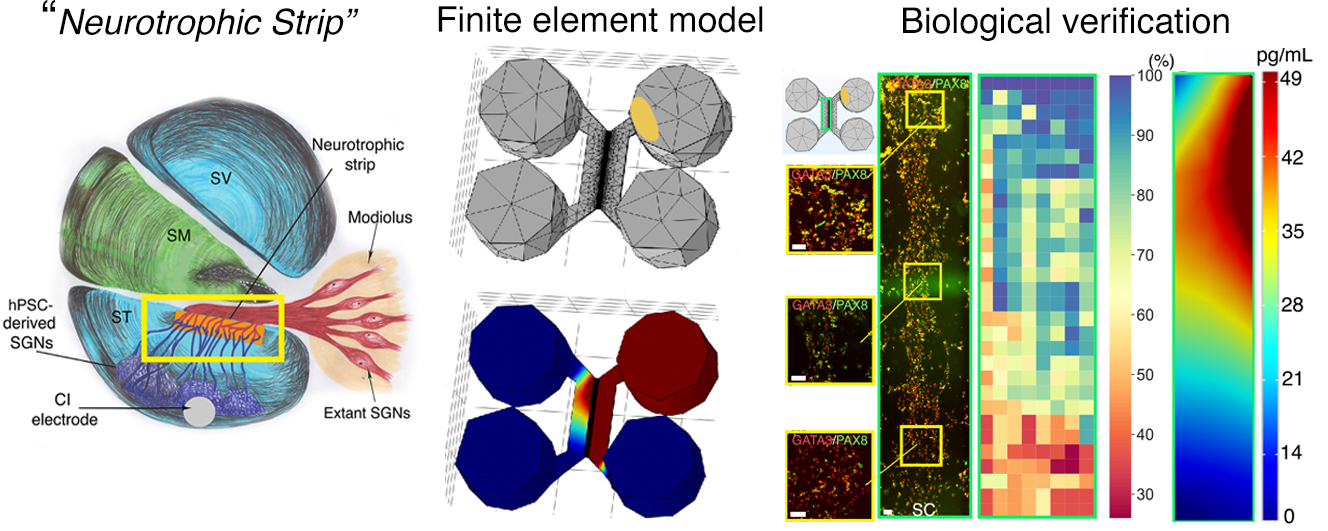
\includegraphics[width=\textwidth]{Graphical_Abstract.jpg}
\end{graphicalabstract}

\begin{keyword}
	human pluripotent stem cells \sep finite element model \sep microfluidic device \sep neurotrophic factor \sep cochlear implant \sep neuroelectric interface \sep stem cell niche \sep spiral ganglion neurons
	\MSC[2010] 74S05 \sep 62P10 \sep 92C20 % I am not sure if you guys need these for this particular journal. 
\end{keyword}
\newpageafter{keyword}

\end{frontmatter}
\newpage

\linenumbers

%%%%%%%%%%%%%
%INTRODUCTION
%%%%%%%%%%%%%
\linenumbers
\clearpage
\pagenumbering{gobble}
\section{Introduction}
\indent The cochlear implant (CI), which provides functional restoration in patients with sensorineural hearing loss, forms a neuro-electronic interface with the peripheral auditory nervous system \cite{Naples2020a}. CI technology functions by electrically stimulating the extant population of auditory neurons (i.e., spiral ganglion neurons [SGNs]). Although CI technology has allowed partial restoration of hearing for this patient population over the last few decades, persistent challenges, including the deciphering of rich acoustic signals into digital pulse-train signals, remain. Among these challenges, the “electrode-neuron gap” poses the most significant obstacle to advancing past the current plateau in CI performance. This phenomenon symptomatically manifests as limited performance in noisy environments and poor ability to decode intonation and music \cite{Wilson2008a}, arguably decreasing quality of life. The gap exists between the CI electrode and the target membranes of dendrites in surviving endogenous SGNs \cite{Frick2017}. It results in the requirement of larger CI excitation fields, leading to current spread that excites and therefore disables the neighboring electrodes, resulting in fewer information channels to the brain, all within discrete time steps \cite{Wilson2008a, Hahnewald2016}. This can develop into a vicious cycle as fewer information channels to the brain also prompt the need for larger CI excitation fields. The length of the gap generally spans hundreds of $\mu$m \cite{Shepherd1993, Tykocinski2000}. Hahnewald et al. demonstrated \textit{in vitro} that energy needed to elicit a response can be reduced by up to 20\% by reducing the distance from 40 to zero $\mu$m (by growing early postnatal mouse SGN explants on a microelectrode array) \cite{Hahnewald2016}.

\indent Previous work has introduced the concept of a "bioactive" CI to resolve the electrode-neuron gap \textit{in vivo}\cite{Roemer2016a, Heuer2021, Chang2020}. The bioactive CI combines the current state-of-the-art CI technology with emerging stem cell–replacement therapy in the inner ear. In this scheme, transplanted human pluripotent stem cell (hPSC)-derived SGNs bridge the gap between the CI electrode and surviving endogenous SGNs. Furthermore, introducing neurotrophin gradients has been shown to guide hPSC grafts in spinal cord injury \cite{Taylor2006}, direct growth of endogenous SGNs toward CI electrodes in the scala tympani \cite{Senn2017}, and enable transplanted hPSC derived otic neuronal progenitors (ONPs) to grow neurites toward the modiolus \cite{Chang2020}. Although promising, these studies failed to observe adequate directed neurite outgrowth toward endogenous SGNs (i.e., lack of synaptic connections between hPSC grafts and endogenous SGNs), presumably preventing significant improvements in functional recovery of hearing.

%%%%%%%%%%
%Figure 1%
%%%%%%%%%%
\begin{figure}
	\begin{center}
		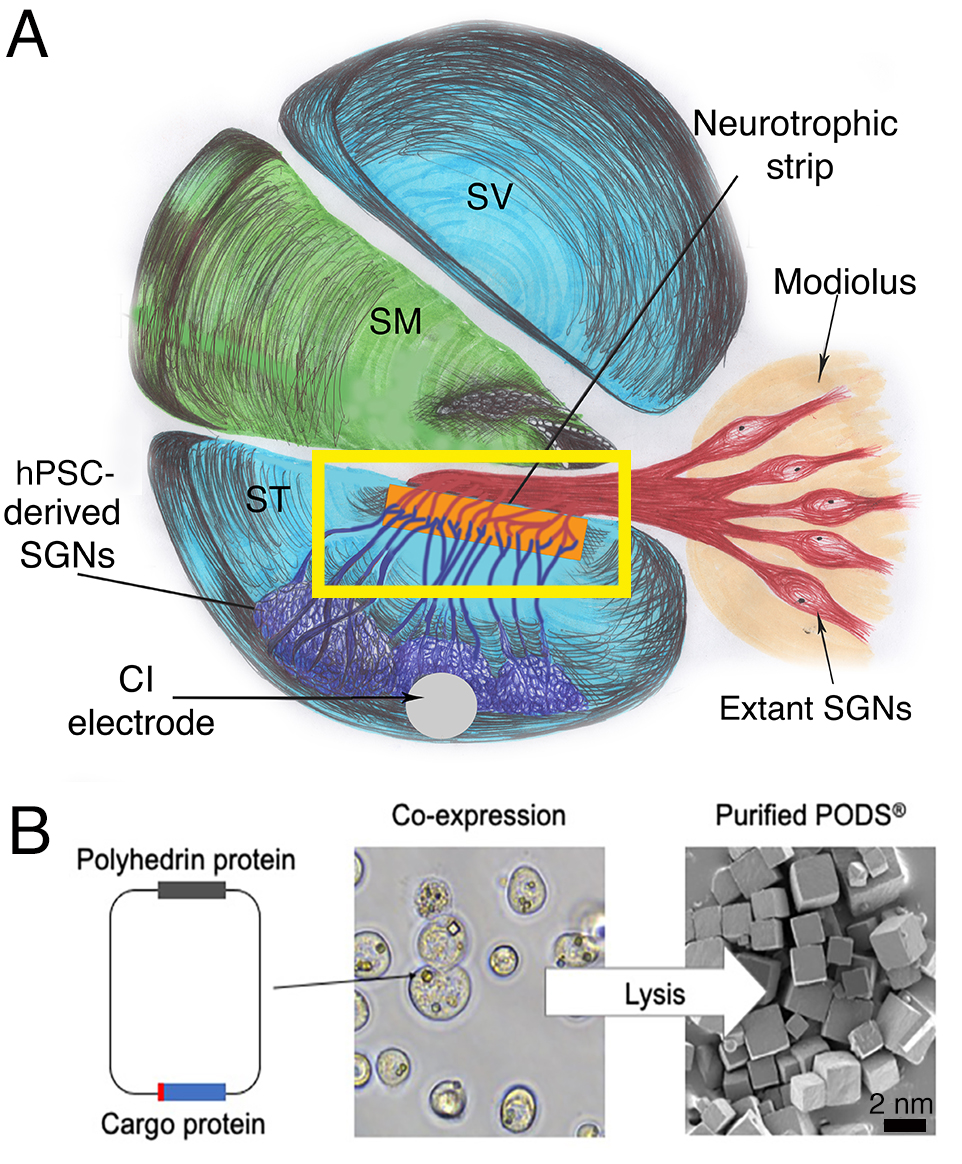
\includegraphics[width=\textwidth]{Fig_1.jpg}
	\end{center}
	\caption{
		(A): A next-generation bioactive CI and a neurotrophic strip. The neural network in this scheme consists of a CI electrode, transplanted stem cell-derived SGNs, the neurotrophic strip, and extant/endogenous SGNs (red). Note that neuronal connection is largely absent with hair cells (not shown). (B): Polyhedrin Delivery System (PODS)\textsuperscript{\textregistered}. PODS\textsuperscript{\textregistered} crystals are cubic protein co-crystals produced by Sf9 cells (a clonal isolate of \textit{Spodoptera frugiperda} Sf21 cells [IPLB-Sf21-AE], in which the polyhedrin protein and a second protein are co-expressed). This second protein is termed as the active, or cargo protein (Figure 1B, left). Inside the Sf9 cells, polyhedrin proteins self-assemble in to cubic crystals (Figure 1B, center) while the active protein, tagged with a short peptide sequence, bind to the growing polyhedrin crystal. The crystals are extracted and purified by simple cell lysis and washes to removed cell debris (Scanning electron micrograph, Figure 1B, right).
	}
\end{figure}

\indent To confront this issue, we propose the development of a “neurotrophic strip”\textemdash a biological interface that doubly preserves endogenous SGNs and precisely directs the growth of neurites arising from transplanted hPSC-derived ONPs toward the endogenous SGNs. The highlighted yellow-square area in Figure 1A shows a schematic diagram of this concept. Here, the neurotrophic strip (shown as an orange rectangle in Figure 1A) stimulates neurite outgrowth from both the hPSC-derived ONPs and the endogenous SGNs via a neurotrophic factor gradient \cite{Goodhill1998}. While the concept of using a neurotrophin gradient for directional axonal growth has existed for a few decades, incorporation of neurotrophin gradients with any tissue- or bio-engineered scaffold has been extremely challenging due to the lack of self-sustaining neurotrophin delivery methods—their eventual depletion triggers an accelerated decline in neurite growth and survival of extant SGNs \cite{Gillespie2003, Pettingill2008, Shepherd2009}. One major contributor is the structurally unstable nature of neurotrophins, which suffer from fragility and thermo-instability under normal physiological conditions both \textit{in vitro} and \textit{in vivo}, leading to short half-lives typically ranging from minutes to hours \cite{Baseri2012}. We set out to mitigate this phenomenon by utilizing the polyhedrin delivery system (PODS\textsuperscript{\textregistered})\textemdash a crystalline growth factor formulation developed to enable long-term release of growth factors (e.g., neurotrophins) \cite{Ikeda2001a,Suzuki1997,Mori1993} (Figure 1B). The PODS\textsuperscript{\textregistered} technology has adapted viral machinery to encase a chosen growth factor into polyhedrin protein cases.The resultant growth factor co-crystals have slow degradation profiles under physiological conditions and, therefore, allow the sustained release of embedded bioactive growth factors.  

\indent We reasoned that a bio-engineered scaffolding incorporated with PODS\textsuperscript{\textregistered} technology can establish a neuronal network between transplanted hPSC-derived ONP grafts and extant SGNs in the inner ear. More specifically, we hypothesized that PODS\textsuperscript{\textregistered}-recombinant human neurotrophin system could stably provide and maintain an adequate neurotrophin gradient to facilitate otic neuronal differentiation of and directional neurite outgrowth from hPSC-derived ONPs, . To test this hypothesis, we first devised a finite element model (FEM) to simulate the \textit{in vitro} neurotrophin gradient generated by PODS\textsuperscript{\textregistered}. In this study, we focus on the role of BDNF\textemdash the most studied of the neurotrophins in the inner ear, and the most vital for the functional recovery of damaged SGNs \cite{green2012}. For biological validation and demonstration we used a multi-chamber microfluidic device, that which mimics the \textit{in vivo} micro-environment of the inner ear more so than conventional laboratory plates in terms of volume and concentrations of endogenous/exogenous factors \cite{Meyvantsson2008}. 

%%%%%%%%%%%%%%%%%%%%%%%
%Materials and Methods
%%%%%%%%%%%%%%%%%%%%%%%
\section{Materials and Methods}
\subsection{Polyhedrin delivery system}
The Polyhedrin Delivery System (PODS\textsuperscript{\textregistered}-human BDNF [rhBDNF]) (Cell Guidance Systems, Cambridge, United Kingdom) was used as a self sustaining source of rhBDNF. PODS\textsuperscript{\textregistered}-rhBDNF is composed of the polyhedrin protein formed by \textit{Bombyx mori}, an insect from the moth family \textit{Bombycidae}. A cargo protein (i.e., rhBDNF) is co-expressed within the polyhedrin crystal and is slowly released by breakdown of the PODS\textsuperscript{\textregistered} crystals via cell-secreted proteases (Figure 1B)\cite{Chang2020, Suzuki1997, Guo2017}. 

\subsection{Human pluripotent stem cell culture using dual-compartment microfluidic device}
Human embryonic stem cells (hESCs: H7 and H9, passages number 25\textendash 35) and were obtained from WiCell Research Institute (Madison, Wisconsin, USA). Human induced pluripotent stem cells (hiPSCs:  TC-1133HKK, passage number 22\textendash 35) were generated from human CD34+ cord blood cells using the four Yamanaka factors at Lonza (Walkersville, Maryland [MD], USA). The hiPSC cell line (TC-1133HKK) was kindly provided by Healios K.K. (Tokyo, Japan). hPSC-derived ONPs were derived based on our previously established protocol (Supplemental Data) \cite{Heuer2021,Chang2020, Matsuoka2017g, Matsuoka2017}. A step-wise series of ligands and growth factors was added to a neuronal induction medium to promote hPSC differentiation toward the late-stage ONP lineage\textemdash mitotic progenitor population that generates the SGNs. (Figure 2).

%%%%%%%%%%
%Figure 2% 
%%%%%%%%%%
\begin{figure}
	\begin{center}
		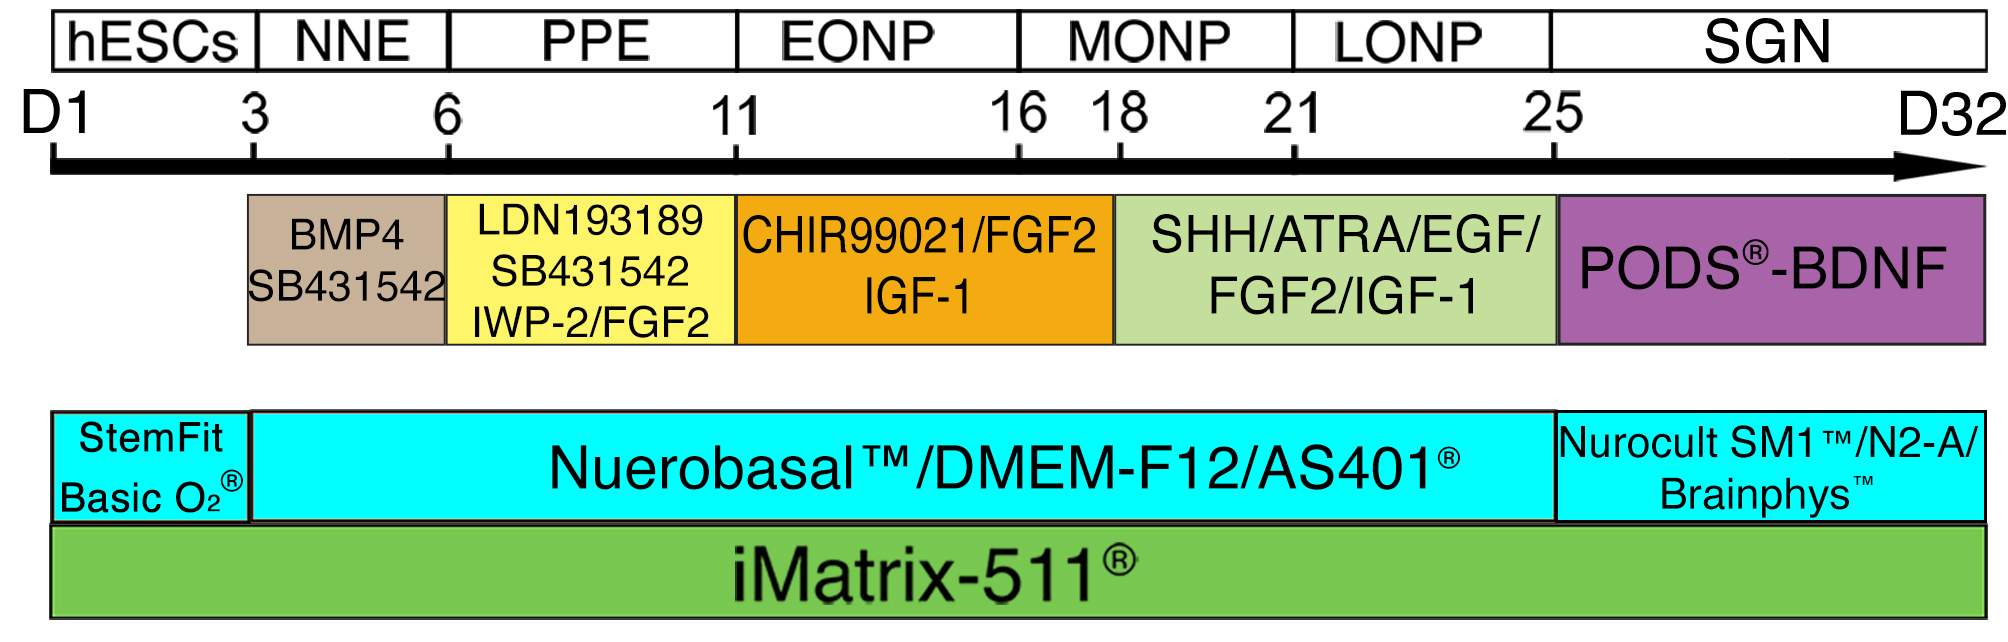
\includegraphics[width=12cm]{Fig_2.jpg} %original figure = Figure_3_layered.psd
	\end{center}
	\caption{Overview of otic neuronal differentiation protocol for hPSCs. Please see detail in \cite{Heuer2021, Chang2020,Matsuoka2017g, Matsuoka2017} and the Supplemental Data. Each developmental stage is shown at the top, with key treatments shown below. NNE: nonneuronal ectoderm; PPE: preplacodal ectoderm; EONP: early-stage otic neuronal progenitor; MONP: mid-stage otic neuronal progenitor; LONP: late-stage otic neuronal progenitor; BMP4: bone morphogenetic protein 4; SHH: Sonic hedgehog; ATRA: all-trans retinoic acid; EGF: epidermal growth factor; IGF-1: insulin-like growth factor-1; FGF2: fibroblast growth factor 2; N2B27-CDM: chemically defined medium containing N2 and B27 supplements.}
\end{figure}

Microfluidic devices provide a platform for specifically evaluating axonal regeneration \cite{Al-Ali2017a}. Here, multi-chamber microfluidic devices, Xona\textsuperscript{\texttrademark} Microfluidics XC150 and XC450 (Xona\textsuperscript{\texttrademark} Microfluidics, Research Triangle Park, North Carolina, USA), were used for computational calculation and biological validation (Figure 3A\textendash B) of an FEA. The Xona \textsuperscript{\texttrademark} device allows for neurites to grow toward growth factors in the opposite chamber while limiting migration of derived ONP cell bodies due to specific dimensions of the device. \added{Additionally, the microchannel array between the two chambers mimics the porous bony separation (osseous spiral lamina) between the modiolus (where extant SGNs are localized) and the scala tympani (where the biohybrid CI will be implanted). Thus the diffusion profile of the released rhBDNF \textit{in vitro} more accurately predicts that of the \textit{in vivo}.}

%%%%%%%%%%
%Figure 3%
%%%%%%%%%%
\begin{figure}
	\begin{center}
		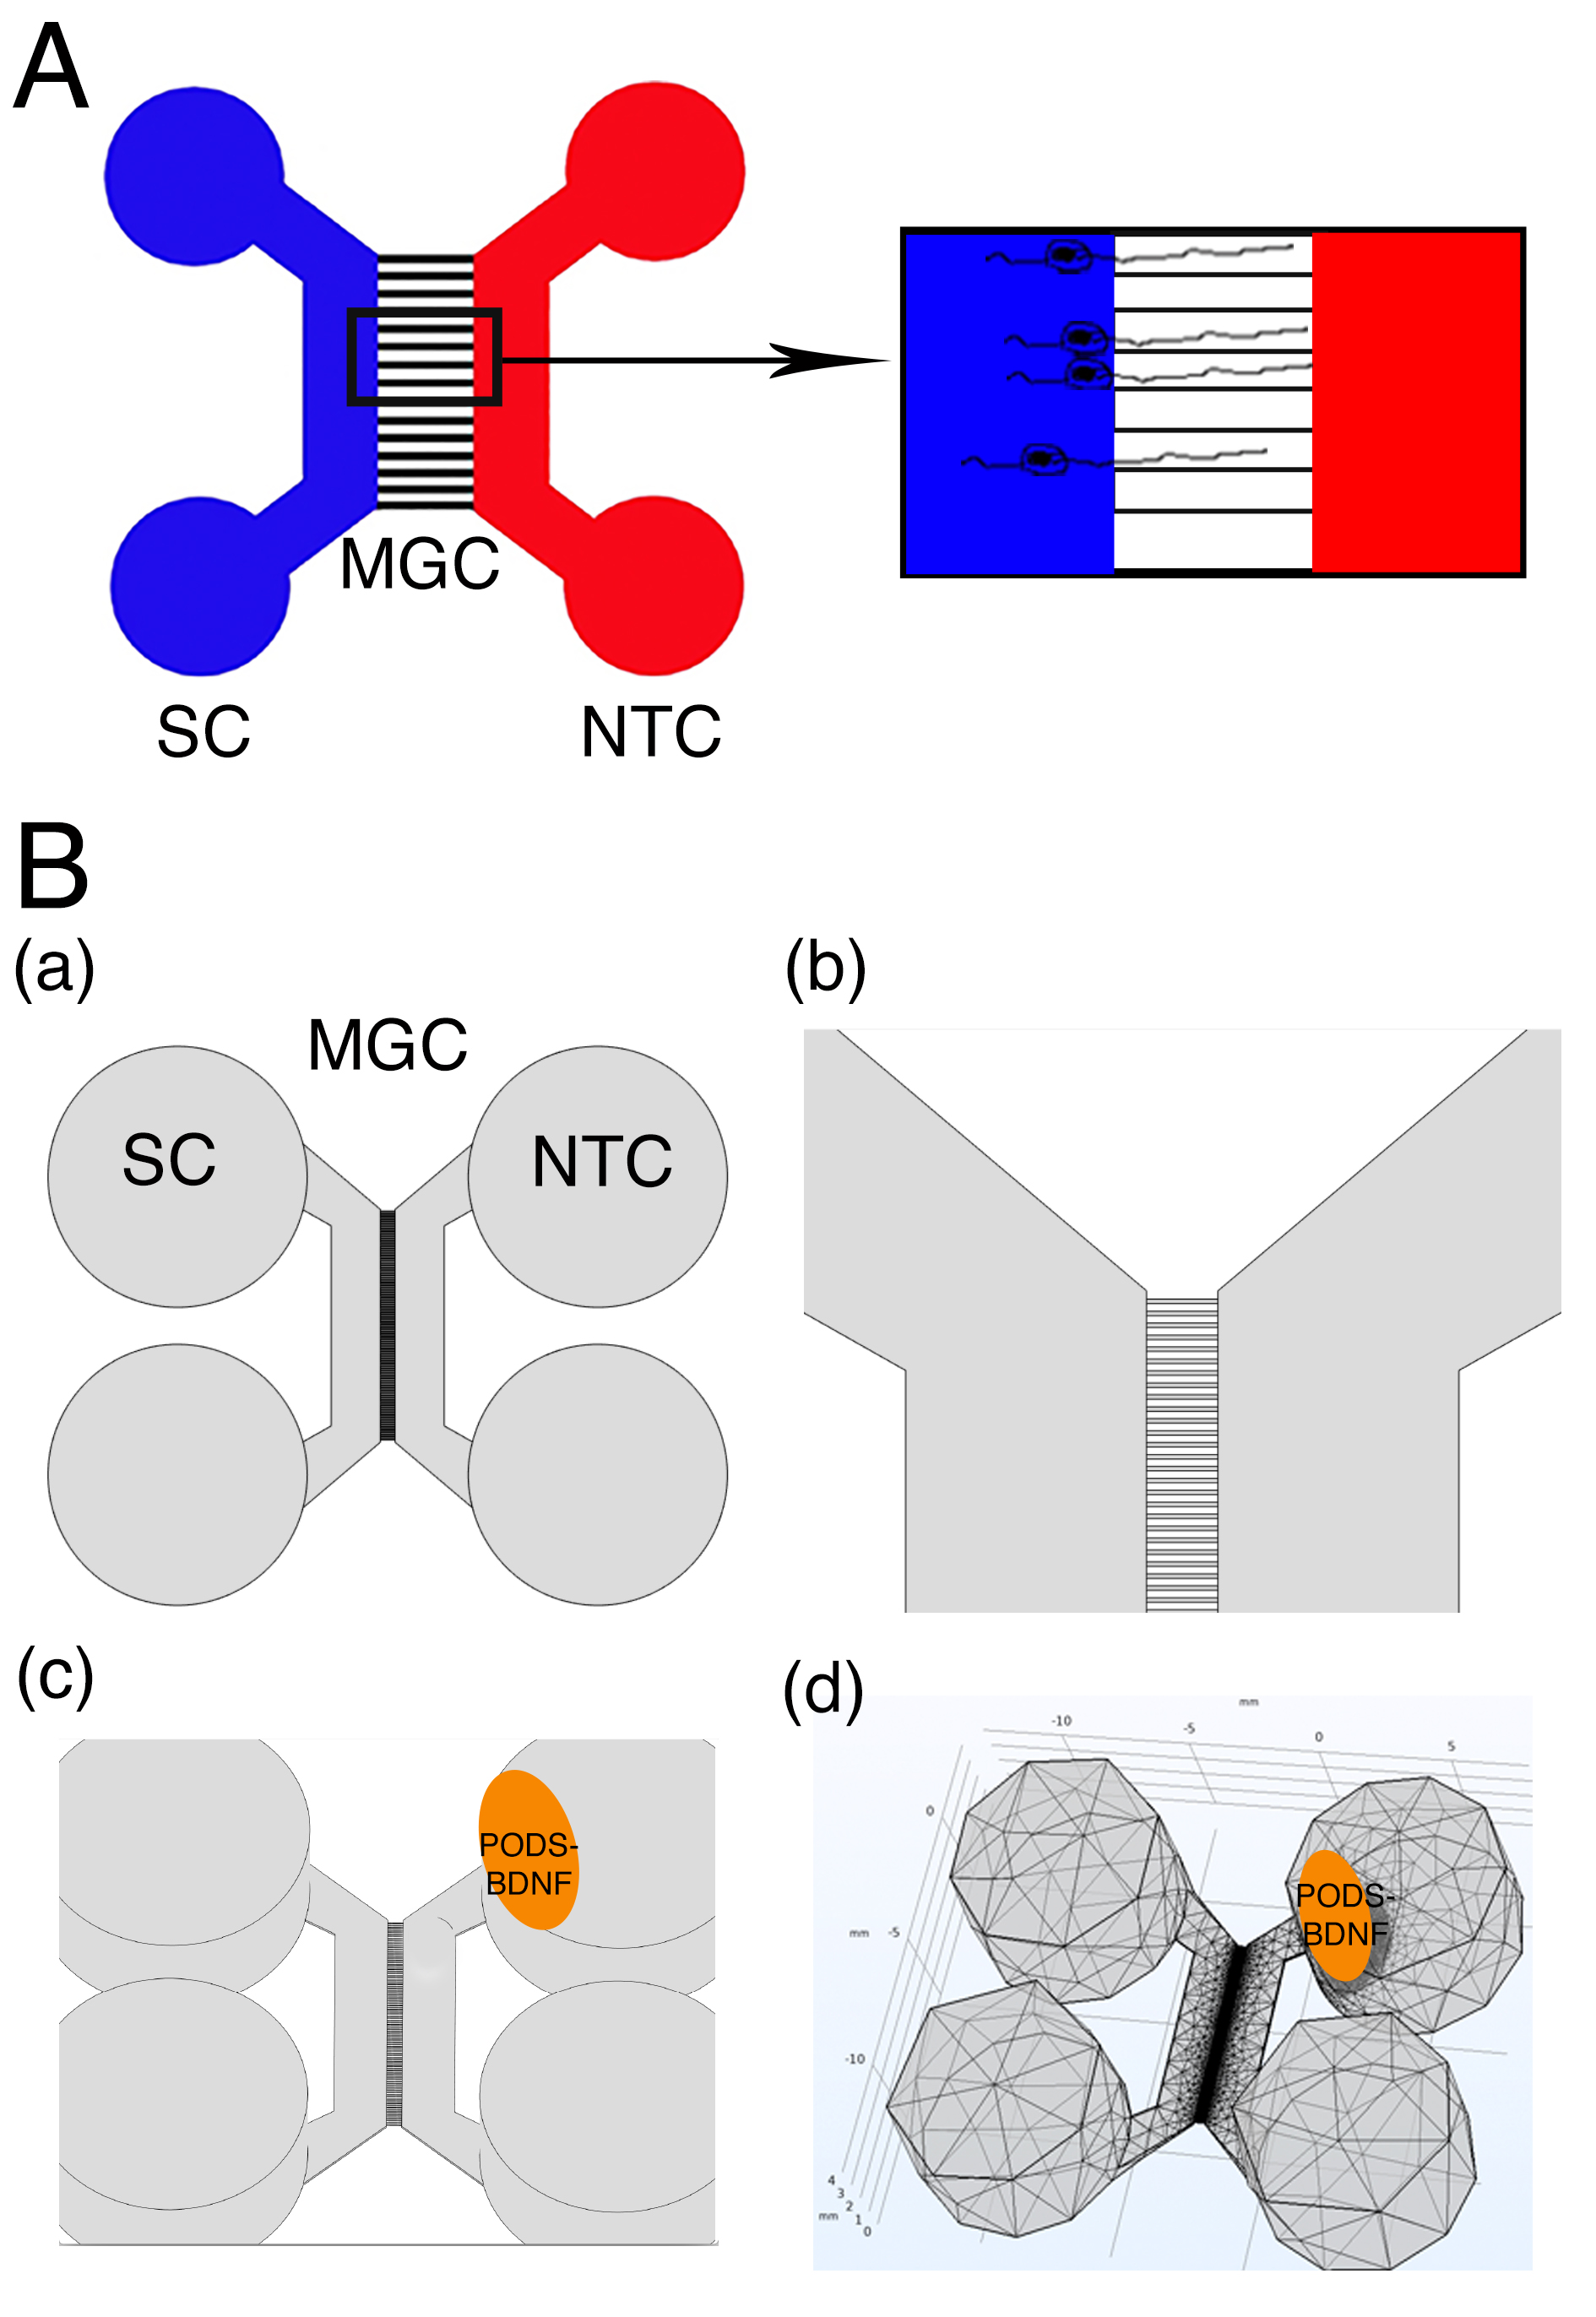
\includegraphics[width=10cm]{Fig_3.jpg} %original figure = Figure_2_layered.psd
	\end{center}
	\caption{(A): Schematic specification of a Xona\textsuperscript{\texttrademark} Microfluidics XC 450. Two main channels (somal compartment (SC) and neurotrophin compartment (NTC)) on either side are connected by a micro-groove channel (MGC) spanning 450 $\mu$m with a width of 10 $\mu$m (black square). The somal compartment contains hPSC-derived late-stage ONPs (shown in black), while the neurotrophin compartment contains the secreted factors (i.e., BDNF) that are released from PODS\textsuperscript{\textregistered}-rhBDNF crystals. (B):(a) Xona \textsuperscript{\texttrademark} Microfluidics XC450 device geometry, created at a 1:1 scale with Autodesk Inventor\textsuperscript{\textregistered}, in which the diffusion profile of the released BNDF was modeled. (b) Detail of the microchannels adjoining the two compartments of the Xona \textsuperscript{\texttrademark} Microfluidics XC450.  (c) Xona \textsuperscript{\texttrademark} Microfluidics XC450 device showing the optimal area and geometry to localize PODS\textsuperscript{\textregistered}-rhBDNF (yellow ellipsoid area). (d): Mesh geometry of the Xona\textsuperscript{\texttrademark} XC450 generated with Autodesk Inventor, depicting the localized volume of PODS\textsuperscript{\textregistered}-rhBDNF (1 $\mu$L) as an ellipsoid disc.}
\end{figure}

The devices were washed and coated with poly-L-ornithine (PLO, 20 $\mu$g/mL in H\lowercase{2}O, Sigma-Aldrich, St. Louis, Missouri [MO], USA) and recombinant laminin-511 (iMatrix-511, 0.5 mg/mL, Nacalai USA, San Diego, California [CA], USA) according to the manufacturer-outlined protocol. Next, approximately 1.75  x 10$^{5}$ cells (in 20 $\mu$L of media) were added through the top and bottom left wells into the somal compartment (i.e., total amount of 3.5 x 10$^{5}$ hPSC-derived ONPs were added). 

\indent PODS\textsuperscript{\textregistered}-rhBDNF were placed in the top right well of the neurotrophin compartment (Figure 3A\textendash B) to generate a rhBDNF concentration gradient to promote directional neurite growth.  hPSC-derived ONPs were cultured for 7 days in the Xona\textsuperscript{\texttrademark} device to induce otic neuronal differentiation. Note that high-density cell cultures were induced to facilitate molecular studies as well as the generation of a more biologically relevant neuronal phenotype (i.e., otic lineage) \cite{Al-Ali2017a}. Media was topped off daily after imaging (from 20-40 $\mu$L per well).

\subsection{Enzyme-linked immunosorbent assay for brain-derived neurotrophic factor}
In order to determine the breakdown and release kinetics of PODS\textsuperscript{\textregistered}-rhBDNF, an experiment measuring rhBDNF concentrations at sequential time points was performed. The culture media from both a control and experimental condition were collected at each time point and immediately stored at -80$^\circ$C before running an enzyme-linked immunosorbent assay (ELISA) after the final collection. The same method was applied to measure the degradation kinetics of rhBDNF protein with a carrier protein (Bovine Serum Albumin [BSA]) (\#248-BDB-050, R\&D Systems, Minneapolis, Minnesota, USA). Experimental conditions were culture media enriched with 10\% fetal bovine serum (FBS) (Thermo Fisher Scientific, Waltham, MA, USA). All rhBDNF samples were quantified with a BDNF ELISA kit (\# BGK23560; PeproTech, Rocky Hill, New Jersey, USA), and the results were analyzed with a Synergy HTX Multi-Mode Reader (BioTek, Winocski, Vermont, USA) at a 450 nm wavelength, as instructed by the manufacturer. Molecular kinetics were then calculated using the MATLAB Curve Fitting Toolbox (MathWorks, Natick, CA, USA).

\subsection{Sodium dodecyl sulphate–polyacrylamide gel electrophoresis} 
Sodium dodecyl-sulfate polyacrylamide gel electrophoresis (SDS-PAGE) is commonly used as a method to separate proteins with molecular masses between 5 and 250 kDa  \cite{Laemmli1970}, a range of which is suitable for detecting recombinant human BDNF (molecular weight [MW]: 14kDa \cite {Mandel2009}) and polyhedrin (MW: $\sim$29 kDa \cite{Guo2017}). In this study, SDS-PAGE was used to assess the molar ratio of polyhedrin to BDNF at different quantities.  Briefly, each protein sample was diluted in deionized water and mixed with 6x Laemmli sample buffer (Bio-Rad Laboratories, Inc., Des Plaines, Illinois [IL], USA) containing 2-mercaptoethanol and heated at 100$^\circ$C for 5 to 20 minutes. Samples were then loaded into precast Mini-PROTEAN TGX 4-15\% polyacrylamide mini-gels (Bio-Rad Laboratories, Inc., Des Plaines, IL, USA). Then, 5 mL of Precision Plus Protein Kaleidoscope Prestained Protein Standards (Bio-Rad Laboratories, Inc., Des Plaines, IL, USA) were loaded in each gel run. Electrophoresis was performed at room temperature for approximately 90 minutes using a constant voltage (100V) in 1x solution of Tris-Glycine-SDS electrophoresis buffer (Bio-Rad Laboratories, Inc., Des Plaines, IL, USA) until the dye front reached the end of the 60 mm gel. After electrophoresis, the mini-gels were rinsed with deionized water 3 times for 5 minutes and were subsequently incubated in SimplyBlue\textsuperscript{\texttrademark} SafeStain (ThermoFisher Scientific, Waltham, MA, USA) for one hour at room temperature with gently agitation. Images obtained from gels were analyzed using ImageJ 1.53g (December 4, 2020, the National Institutes of Health, Bethesda, MD, USA \cite{Schneider2012}). The calculated molar ratio was applied to the COMSOL\textsuperscript{\textregistered} Multiphysics model to accurately predict the amount of rhBDNF released from PODS\textsuperscript{\textregistered}-rhBDNF. SDS-PAGE was performed according to the manufacture's technical guide (Bio-Rad Laboratories, Inc., Des Plaines, IL, USA). 

\subsection{Western Blot} 
The identity of the rhBDNF protein detected by SDS-PAGE was verified by western blot (Bio-Rad Laboratories, Inc., Des Plaines, IL, USA). Briefly, the polyvinylidene difluoride (PVDF) membrane was prepared in methanol for 30 seconds before soaking in 1x Tris-Glycine-Methanol transfer buffer for 10 minutes. Wet transfer was performed at 4$^\circ$C for approximately 60 minutes using a constant voltage (100V) in 1X solution of Tris-Glycine-Methanol transfer buffer. After transfer, the membrane was briefly rinsed with 1X Tris-buffered saline Tween-20 (TBST) and was subsequently blocked in 5\% BSA in TBST for 24 hours at 4$^\circ$C with gentle agitation. The membrane was then rinsed with 1x TBST before incubating in BDNF polyclonal antibody (ThermoFisher Scientific, Waltham, MA, USA) diluted to 1:1500 in 1\% BSA in TBST for 24 hours at 4$^\circ$C with gentle agitation. Following incubation, the membrane was rinsed in 1x TBST 5 times for 5 minutes to remove unbound primary antibody. Then, the membrane was incubated in Goat anti-Rabbit IgG (H+L) horseradish peroxidase (HRP) conjugated secondary antibody (ThermoFisher Scientific, Waltham, MA, USA) diluted to 1:5000 in 1\% BSA in TBST for one hour at room temperature with gentle agitation. Following incubation, the membrane was rinsed in 1x TBST 5 times for 5 minutes to remove unbound secondary antibody. For sensitive detection, the membrane was treated with Pierce\textsuperscript{\texttrademark} ECL Western Blotting Substrate (ThermoFisher Scientific, Waltham, MA, USA), and visualized using an Azure 600 Digital Imager (Azure Biosystems, Dublin, CA, USA). Electrophoresis buffer for sample condition and run condition was summarized in Supplementary Table S1. 

\subsection{Three-dimensional finite element analysis}
We used finite element analysis (FEA) to simulate the BDNF concentration gradient over time in a multi-chamber microfluidic device. FEA is a computational numerical technique, which approximates mathematical solutions to partial differential equations (PDEs) that appropriately simulate complex real-world problems including stress/strain testing, thermal conduction, and diffusion in various geometries and materials. In this study, the FEM allowed us to predict the concentration gradient with respect to time depending on the number of PODS\textsuperscript{\textregistered}-rhBDNF introduced into the system. To solve the FEM, we used COMSOL\textsuperscript{\textregistered} Multiphysics (version 5.6 [released on November 11, 2020], COMSOL, Inc., Burlington, Massachusetts [MA], USA), which is a finite element method solution tool for engineering and scientific research computations. We used sustained-release kinetics for PODS\textsuperscript{\textregistered}-rhBDNF determined from aforementioned ELISA studies, SDS-PAGE, as well as data from a previous study from our group \cite{Chang2020}. Device geometry was generated at a 1:1 scale using Autodesk\textsuperscript{\textregistered} Inventor 2019.0.2 (Autodesk, Mill Valley, CA, USA) (Figure 3B). The computational analysis was implemented on a high-performance desktop computer platform equipped with a 64 GB RAM CPU (AMD Ryzen Threadripper 3990X 64-Core, 128-Thread @ 4.3 GHz) and two GPU cards (NVIDIA GeForce RTX 3080Ti,12GB 384-bit GFF6X Graphics card).

\subsection{Immunocytochemistry and image acquisition}
Microfluidic devices were coated with poly-d-lysine (PDL) (\#A3890401, ThermoFisher Scientific, Waltham, MA, USA) and poly-ornithine (PLO) (\# A-004-C, MilliporeSigma, St. Louis, MO, USA) as per the manufucturer’s instructions. A total of 100,000 dissociated hPSC-derived ONPs were plated into the somal compartment of the device. On Day 7, 4\% (w/v) paraformaldehyde (PFA) (ThermoFisher Scientific, Waltham, MA, USA) was added to the compartments for 20 minutes to fix the cells. ICC was used to stain for GATA3, PAX8, and beta-III tubulin. These three proteins have shown to appropriately characterize ONPs in our previous studies \cite{Heuer2021, Chang2020, Matsuoka2017}. Following PBS wash, cultures were blocked with 5\% BSA at room temperature for 1 hour. Cultures were then incubated overnight at 4$^\circ$C on a shaker plate in primary antibody solution using Rabbit anti-Beta-III-Tubulin (1:100, Abcam, Cambridge, MA, USA), Goat anti-PAX8 (1:500, Abcam, Cambridge, MA, USA), and Mouse anti-GATA3 (1:500, R\&D Systems, Minneapolis, MN, USA). Following PBS washes, cultures were incubated at room temperature for 90 minutes on a shaker plate in secondary antibody solution composed of Alexafluor647 anti-Rabbit (1:1000, ThermoFisher Scientific, St. Louis, MO, USA), Alexafluor488 anti-Goat (1:1000, ThermoFisher Scientific, St. Louis, MO, USA), and Alexafluor594 anti-Mouse (1:1000, ThermoFisher Scientific, St. Louis, MO, USA) in 1\% BSA. Following PBS -/- washes, cultures were incubated with DAPI for 20 minutes (300 nM, ThermoFisher Scientific, St. Louis, MO, USA). Secondary antibody controls were performed each time multiple primary antibodies were used \cite{Burry2011}. Labeling controls (detection controls) were performed for a sample from each batch of hPSC culture \cite{Burry2011}. See Supplementary Figure S1 for exemplary figures for these control conditions. Results were imaged using a Nikon Ti2 Widefield Laser Microscope System (Nikon, Tokyo, Japan). Phase-contrast images were captured on a Nikon Eclipse TE2000-U inverted microscope (Nikon, Tokyo, Japan). All fluorescence images were acquired on a Zeiss LSM 510 META laser-scanning confocal microscope (Carl Zeiss, Oberkochen, Germany), a Nikon Ti2 laser laser-scanning confocal microscope (Nikon, Tokyo, Japan), or a Leica SP5 laser-scanning confocal microscope (Leica, Welzlar, Germany). Observers were blinded to the conditions during imaging and tracing. In general, the images were processed with a Image J  ver. 1.53j or Matlab R2020b. Further detail on image acquisition and quantification of fluorescent-positive cells can be found in the Supplemental Data. 

\subsection {Preferred cell orientation analysis}
Collective cell migration, where cells organized in a tightly connected fashion migrate as cohesive structures, is a critical biological process to highlight the neurotrophin diffusion profile \cite{Mazalan2020}. To evaluate this process, time-lapse acquisition of images of the Xona\textsuperscript{\texttrademark} device was performed using an inverted microscope (Nikon Eclipse TS100, Tokyo, Japan) at Day 1, 3, 5, and 7. Due to the high cell density required for hPSC-ONPs to survive in the somal compartment of the Xona\textsuperscript{\texttrademark} device, images were not amenable to manual analysis in most of the cases. To circumvent this problem, we performed a series of image pre-processings that are mainly based on modified binarization-based extraction of aliment score methods with some modifications \cite{Xu2011}. We used MATLAB Image Processing Toolbox R2020b (version 9.9.0.1495850, September 30th, 2020, Mathorks, Natick, MA) for analysis. Please see Supplementary Figure S2 for further detail. The analysis of directional data in general represents a particular challenge: there is no reason to designate any particular point on the circle as zero, and it is somewhat arbitrary depending on where one sets a coordinate \cite{Batschelet1981,Berens2009}. In this study, we used polar coordinates to determine the directionality of preferred cell orientation.  For this analysis, we again used MATLAB Image Processing Toolbox R2020b. See detailed discussion on how we determined the preferred cell orientation in Supplementary Figure S3.

\subsection{Neurite alignment vector assay, neurite growth assay and cell migration assay}
The microfluidic device allowed us to culture hPSC-derived ONPs in a polarized manner and to directly isolate/analyze neurites. To evaluate the neurite projection into the neurotrophin compartment by derived otic neurons cultured in the somal compartment, we performed a neurite alignment vector assay. We also evaluated the length of neurites that grew from hPSC-derived ONPs. For these purposes, hPSC-derived ONPs were cultured in a Xona\textsuperscript{\texttrademark} XC450 for seven days and then immunostained with $beta$-III tubulin and DAPI. We used two ImageJ plug-in toolkits, NeuriteTracer and NeuronJ, to assess neurite alignment and neurite growth \cite{Pool2008, Meijering2004}. Due to the bipolar nature of hPSC-derived ONPs/SGNs, we measured the two longest neurites from the cells \cite{Matsuoka2017,Anniko1995}. Please see Supplementary Figure S4 for detailed description of this analysis. We used hPSC-derived ONPs cultured with 800,000 PODS\textsuperscript{\textregistered}-rhBDNF as a positive control. The quantity 800,000 was chosen based on our FEM in that there was no neurotrophin gradient in the somal compartment. As a negative control, we used 20 ng/mL of recombinant human BDNF. To evaluate cell migration across the microgroove channels, we performed cell migration analysis. We manually counted the number of ONPs that migrated from the somal compartment into the microchannels and neurotrophin compartment. 

\subsection{Statistical analysis}
When appropriate, and as indicated in each figure, statistical analysis was performed. Experimental values are typically expressed as mean and standard error (SE). The majority of the statistical analyses were performed with Python 3.9.6. (Python Software Foundation, Wilmington, Delaware, USA). The following libraries were used for the statistical analysis: Scipy, Numpy, Matplotlib, and Seaborn \cite{5725236, hunter2007,Virtanen2020}. Normal distributions were assumed unless mentioned otherwise. $P$ values smaller than 0.05 were considered statistically significant. For circular statistics, we derived the sample mean vector and its polar coordinate. Mean and confidence intervals were calculated. We chose confidence coefficient, $Q$, e.g. $Q = 0.95$. To analyze the axial nature of data, especially to compute the mean vector angle, we doubled each angle and reduced the multiples modulo 360\degree. Please see detailed discussion in Supplementary Figure S3 and S5. The Rayleigh test of uniformity and V-test were performed to determine whether the samples differ significantly from randomness (i.e., where there is statistical evidence of directionality). One-sample test for the mean angle was performed to test whether the population mean angle is statistically different from the given angle. In all of our circular statistics, von Mises distribution was assumed and also verified. Circular statistics were performed using CircStat: A MATLAB Toolbox \cite{Berens2009, Berens2009a}. Please see detailed description of circular statistics in Supplementary Figure S3 and S5. Experiments were done in three biological replicates unless otherwise specified in Figure captions.



%%%%%%%%%%%%%%%%%
\section{Results}
%%%%%%%%%%%%%%%%%


%%%%%%%%%%
% Figure 4
%%%%%%%%%%
% Figure 4 (ELISA Curve fitting)
\begin{figure}
	\begin{center}
		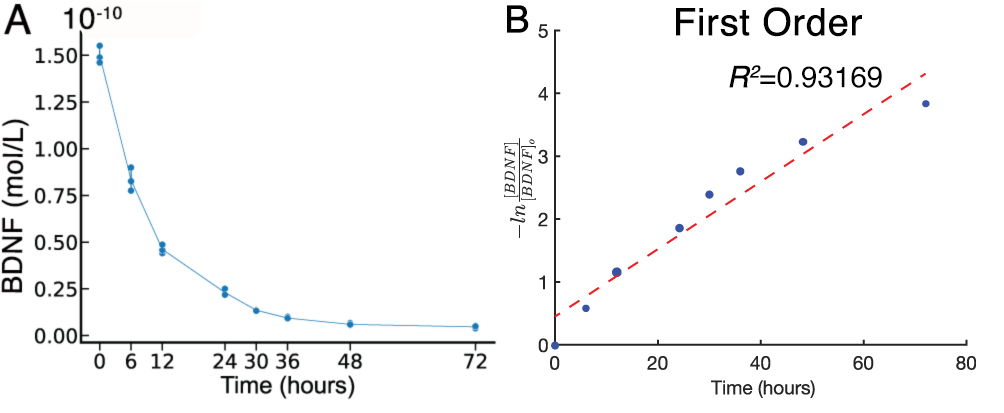
\includegraphics[width=12.5cm]{Fig_4.jpg}
	\end{center}
	\caption{Chemical kinetics of Brain Derived Neurotrophic Factor (BDNF). (A): Concentration of rhBDNF in solution over 72 hours after initial application. (B): $\frac{1}{[BDNF]}$ data fit to first order curve. Please see other curve fit data in Supplemental Figure 1. Red line: fitted line, blue dots: individual data point. $k2$ is defined as slope of fitted curve.} 
\end{figure}

\indent The appropriate number of PODS\textsuperscript{\textregistered}-rhBDNF crystals to induce an effective neurotrophin gradient for otic neuronal differentiation and directed neurite outgrowth was calculated using a three-dimensional FEA that predicts the concentration profile of BDNF formed through the gradual release and diffusion of BDNF from PODS\textsuperscript{\textregistered}-rhBDNF. First, we quantified the chemical kinetics of this phenomenon with ELISA testing (Figure 4) to establish the parameters for the FEA. Here, two consecutive chemical reactions occur: 1) the breakdown of PODS\textsuperscript{\textregistered} crystals into polyhedrin protein and rhBDNF, and 2) the degradation of rhBDNF toward the degradation product (Equation (1)).
%%%%%%%%%%%%%%%
% Equation 1
%%%%%%%%%%%%%%%
\begin{equation}
	PODS\overset{k1}{\longrightarrow}BDNF + PHP\overset{k2}{\longrightarrow}DP + PHP
\end{equation}
%%%%%%%%%%%%%%%
where $DP$ is the degradation product of the released rhBDNF, PHP is the polyhedrin protein, and $k\textsubscript{1}$ and $k\textsubscript{2}$ are the rate constants ($\frac{1}{hour}$) for their respective reactions.


Degradation kinetics data for rhBDNF was collected while monitoring rhBDNF concentration after introducing a predefined amount into a single well of solution. The data obtained throughout the first 72 hours indicate an exponential decay, suggesting first order kinetics (Figure 4). To confirm this notion, we performed a linear and nonlinear least square analysis of the kinetic data with the MATLAB Curve Fitting Toolbox. We found that the corresponding $R^{2}$ was 0.93169 for the first order curve-fit, confirming that the degradation kinetics was indeed first order. The rate constant for a first order reaction is defined to be slope of the time plot of the logarithmic ratio between concentration and initial concentration The value for $k\textsubscript{2}$ ( 0.0679 ($\frac{1}{hour}$) ) is the slope of the logarithm of the ratio between concentration and initial concentration (See further detail in Supplementary Figure S7). Furthermore, data for the complete chemical reaction were collected by similarly monitoring rhBDNF concentration over time after placing a predefined amount of PODS\textsuperscript{\textregistered}-rhBDNF into a single well of solution. The data collected appeared to fit the curve for Equation 2, which describes the concentration of the intermediate product of two consecutive first order reactions:  

%%%%%%%%%%%%%%%
% Equation 2
%%%%%%%%%%%%%%%
\begin{equation}
C_{rhBDNF} =  C_{PODS} \cdot k_1 \cdot (\frac{e^{-k_1 \cdot t}}{ k_2-  k_1}  + \frac{e^{-k_2 \cdot t}}{ k_1 -  k_2} )
\end{equation}
%%%%%%%%%%%%%%%
where $C_{rhBDNF}$ is the concentration of rhBDNF and $C_{PODS}$ is the concentration of PODS\textsuperscript{\textregistered} \cite{levenspiel1999}.

 We successfully fit the data to this equation's respective curve and empirically approximated $k_{1}$ to be 0.00686 ($\frac{1}{hour}$) after plugging in our value for $k_{2}$ (See further detail in Supplementary Figure S7).  
 
 %%%%%%%%%%%%%%%%%%%%%%%%%
 % Figure 5
 %%%%%%%%%%%%%%%%%%%%%%%%%
 % Figure 5 (The Western/SDS-PAGE Figure)
 \begin{figure}
 	\begin{center}
 		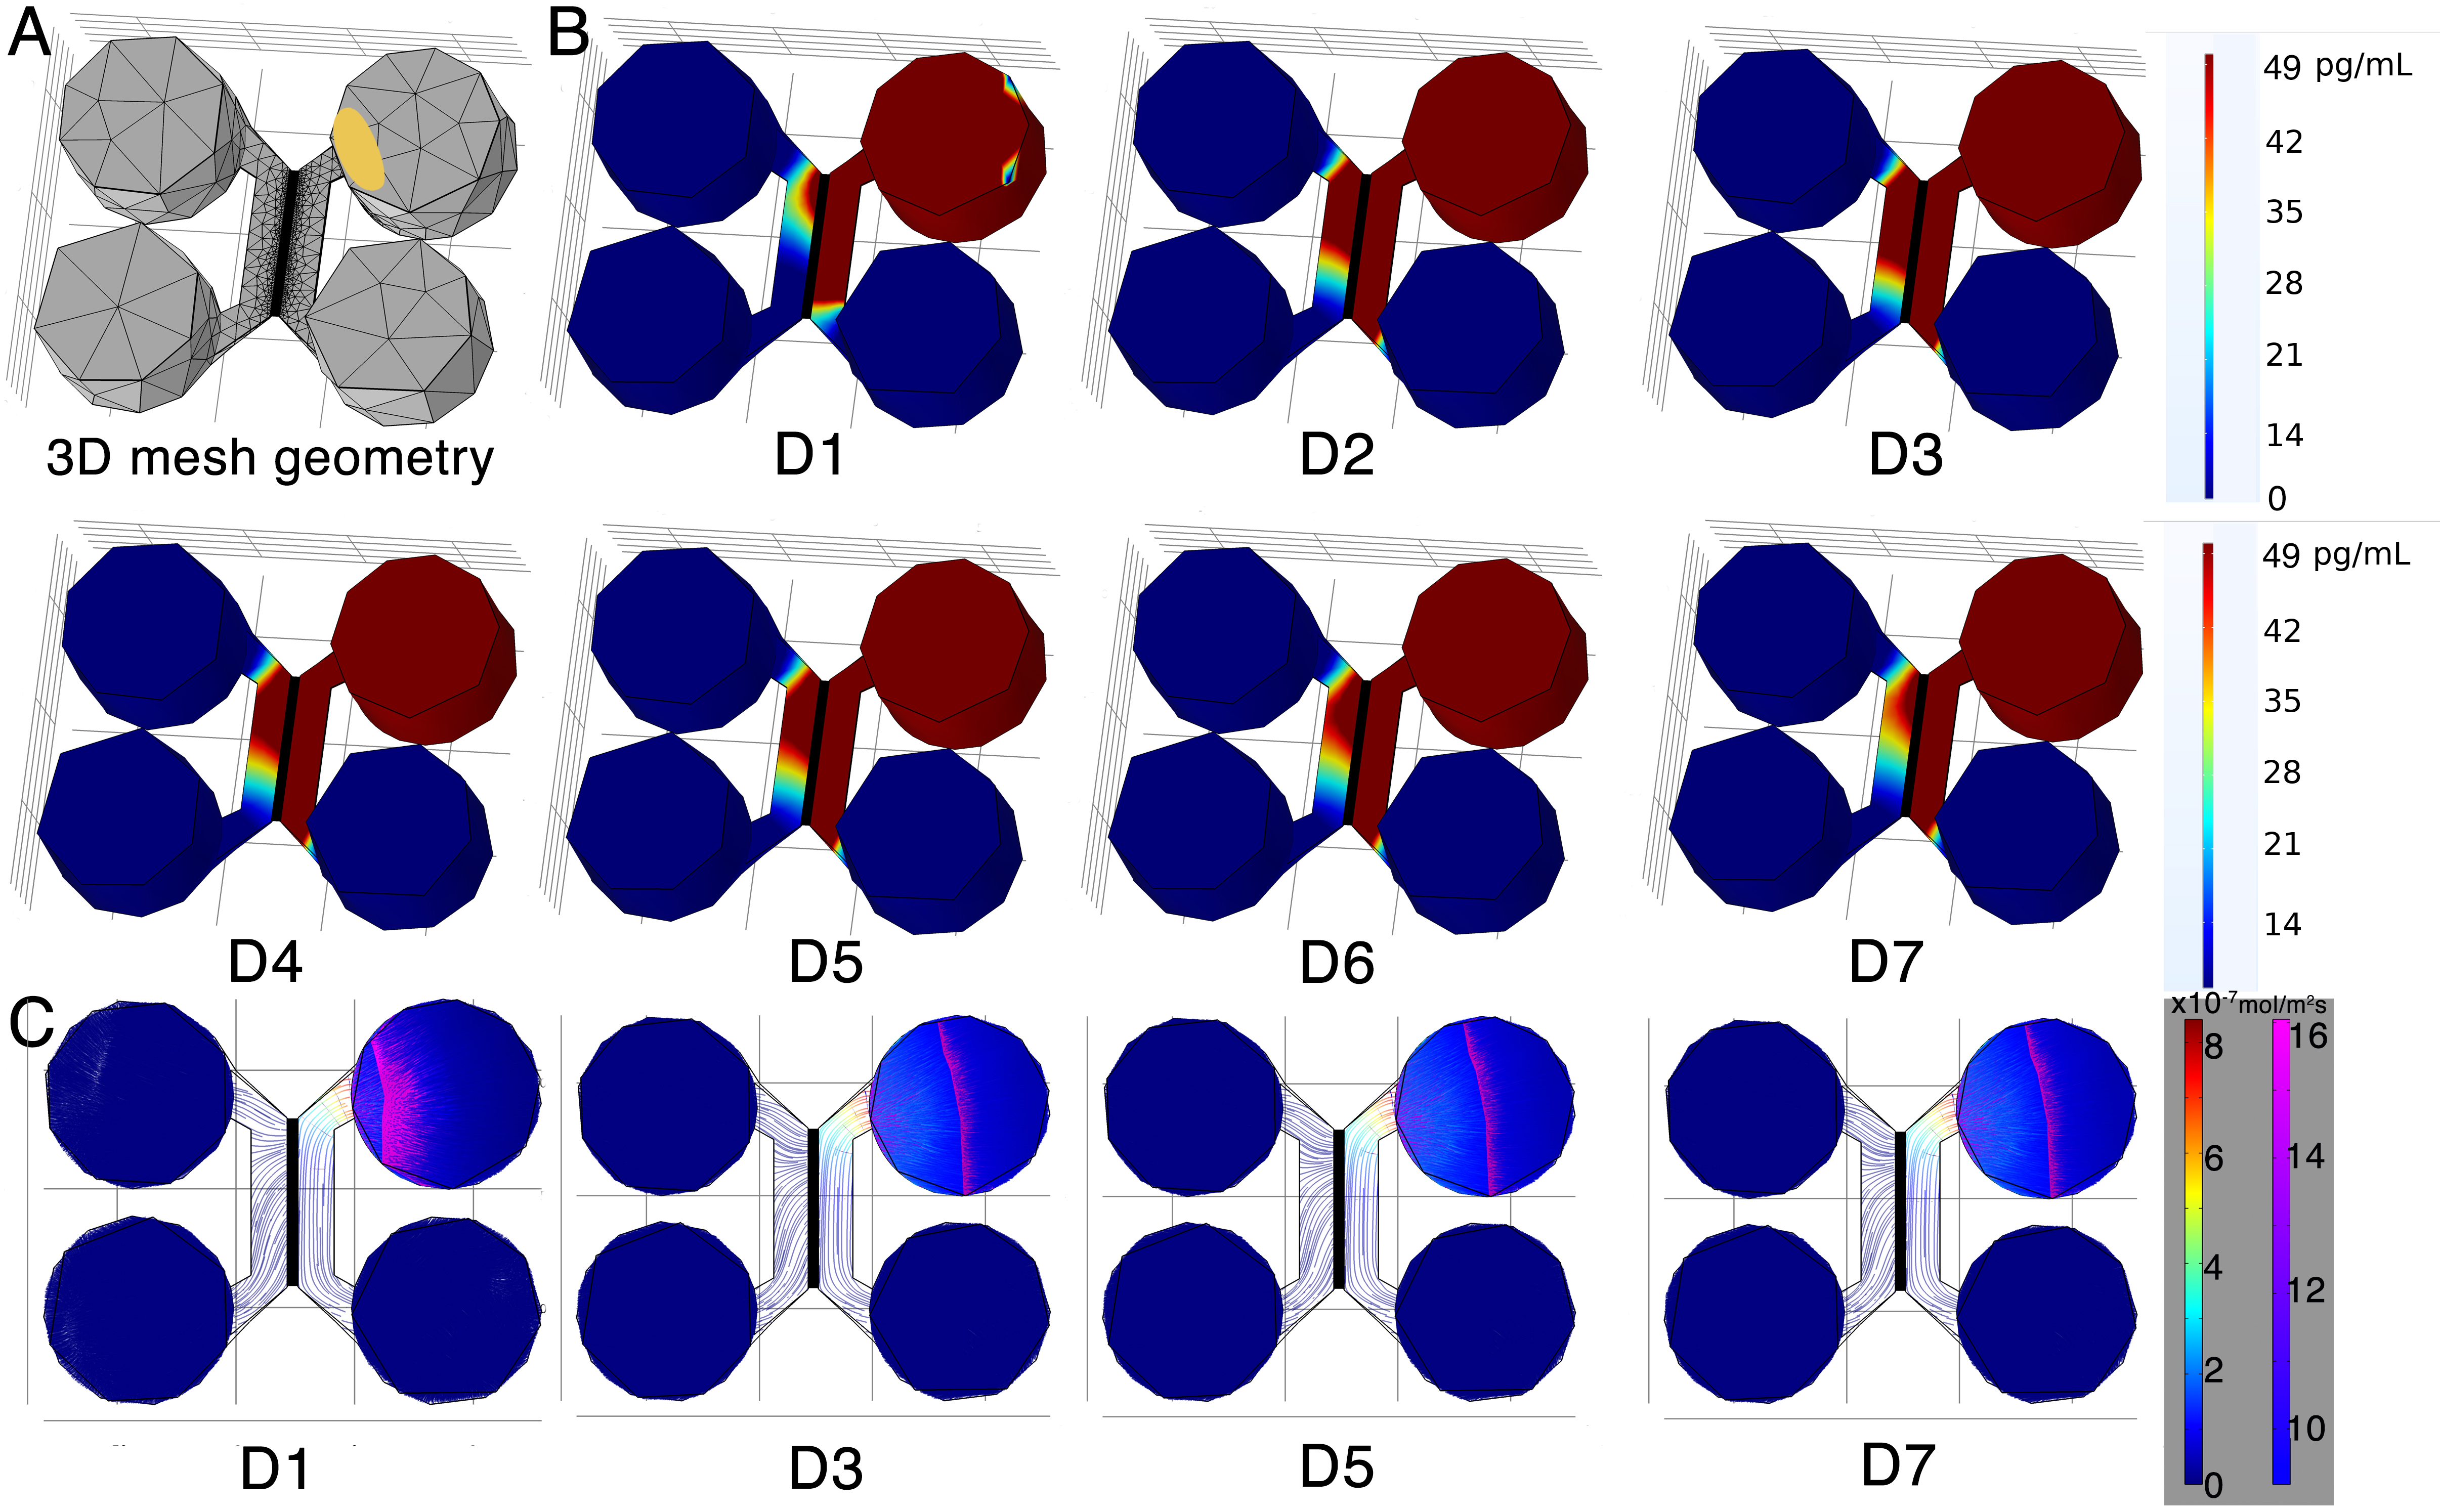
\includegraphics[width=13cm]{Fig_6.jpg}
 	\end{center}
 	\caption{(A): SDS-PAGE analysis of PODS\textsuperscript{\textregistered}-rhBDNF. Samples containing six quantities of PODS\textsuperscript{\textregistered}-rhBDNF crystals were run on precast 4-15\% polyacrylamide mini-gels and stained with Coomassie G-250 solution for visualization. Protein bands appear at approximately 18.8 (a), 28.0 (b), and 46.8 kDa (c). Lane 1: molecular weight marker. Lanes 2-7: samples containing   }
 \end{figure}
 
 
 %%%%%%%%%%%%%%%%%%%%%%%%%%%%%
 %Figure 5 result explanation%
 %%%%%%%%%%%%%%%%%%%%%%%%%%%%%
 SDS-PAGE was used to separate PODS\textsuperscript{\textregistered}-rhBDNF crystals into its constituent proteins to determine the molar ratio of polyhedrin to rhBDNF. Visualization with Coomassie G-250 solution (Figure 6A) revealed three distinct protein bands at 18.8 (a), 28.0 (b), and 46.8 (c) kDa, which correspond with the molecular weights of H1-tagged BDNF monomer, polyhedrin, and H1-tagged BDNF monomer attached with polyhedrin, respectively. Western blot analysis was subsequently conducted to confirm the identity of the 18.8 kDa band as rhBDNF. Enhanced chemiluminescence (Figure 6B) revealed four protein bands at 14.0 (a), 18.8 (b), 37.6 (c), and 46.8 (d) kDa, which correspond with the molecular weights of rhBDNF monomer, H1-tagged BDNF monomer, H1-tagged BDNF dimer, and H1-tagged BDNF monomer attached with polyhedrin. Immunoblot detection of the 18.8 kDa band further implicates its identity as rhBDNF. SDS-PAGE images were converted to 8-bit grayscale and mean corrected integrated pixel intensity values were calculated for protein bands located at 28.0 and 18.8 kDa; the protein band detected at 46.8 kDa was omitted from the final computation based on the fact that it contained a 1:1 ratio of polyhedrin to BDNF. Results indicate that the molecular ratio of polyhedrin to rhBDNF is approximately 22:1. This transforms Equation (1) into:
 
 
 
 %%%%%%%%%%%%%%%
 % Equation 3
 %%%%%%%%%%%%%%%
 %%%%%%%%%%%%%%%
 \begin{equation}
 	PODS\overset{k1}{\longrightarrow}BDNF + 22PHP\overset{k2}{\longrightarrow}DP + 22PHP
 \end{equation}
 %%%%%%%%%%%%%%%

 
 Using these calculated rate constants with the calculated molar ratio, the resulting chemical gradient over time after PODS\textsuperscript{\textregistered}-rhBDNF placement can be solved for any geometry by applying Fick’s second Law of diffusion (Equation 4) and the appropriate boundary (Equations 5 and 6) and initial conditions (Equation 7): 

%%%%%%%%%%%%%%%
% Equation 4
%%%%%%%%%%%%%%%
\begin{equation}
\renewcommand{\vec}[1]{\boldsymbol{#1}}
\frac{dC}{dt}
= \nabla\cdot\left(\nabla C\cdot D\right)-k_{2}\cdot C
\end{equation}

%%%%%%%%%%%%%%%%%%%
% Equation 5 and 6
%%%%%%%%%%%%%%%%%%%
Boundary Conditions:

\begin{equation}
\delta C \Big{|}_{walls}= 0\quad 
\end{equation}

\begin{center}
and
\end{center}

\begin{equation}
\quad\delta C\Big{|}_{PODS}
=k_1 \cdot PODS_0 \cdot e^{-k_1 \cdot t}
\end{equation}

%%%%%%%%%%%%%%%%%%%
% Equation 7
%%%%%%%%%%%%%%%%%%%
Initial conditions: 
\begin{equation}
C\Big{|}_{t=0} = 0
\end{equation}
%%%%%%%%%%%%%%%%%%%%%
where $C$ is the concentration of rhBDNF, $D$ is diffusivity of rhBDNF (6.76 $\frac{mm\textsuperscript{2}}{day} $ \cite{Stroh2004}), $-k\textsubscript{2}\cdot C$ is the sink term corresponding to the degradation and cell-utilization of the rhBDNF, and $PODS_{0}$ is the initial concentration of the cargo protein (i.e., BDNF) within the PODS\textsuperscript{\textregistered} crystals. The first boundary condition (Equation 4) shows that the concentrations of rhBDNF at the walls of the microfludic device are fixed at 0. The second boundary condition (Equation 5) represents the exponential nature of the decay of PODS\textsuperscript{\textregistered}. Note that both are Neumann boundary conditions. 

\indent We empirically tested two available microchannel lengths\textemdash (i.e., Xona\textsuperscript{\texttrademark}-XC150 [150 $\mu$m] and Xona\textsuperscript{\texttrademark}-XC450 [450 $\mu$m]). This was done first because mass (i.e., BDNF) transport from the neurotrophin compartment through the micro-groove channels into the somal compartment is an important factor in generating the concentration gradient \textit{via} diffusion mixing.  We determined that the Xona\textsuperscript{\texttrademark} Microfluidics XC450 was more appropriate for this study as the XC-150's micro-groove channels were not long enough to generate the appropriate concentration gradient throughout the somal compartment. This feature is relevant to human inner ear because the micro-groove channels in the Xona device simulates the presence of the osseous spiral lamina and modiolus between the scala tympani and SGNs  \cite{Tuncel2005,Kucuk1991a}. Following device selection, we generated a three-dimensional geometry mesh of the XC450 for the FEA (Figure 3B(d)). Please see Supplementary Figure S6 for detailed measurements of the mesh. 

%%%%%%%%%%%
% Figure 6
%%%%%%%%%%%%
\begin{figure}
\begin{center}
	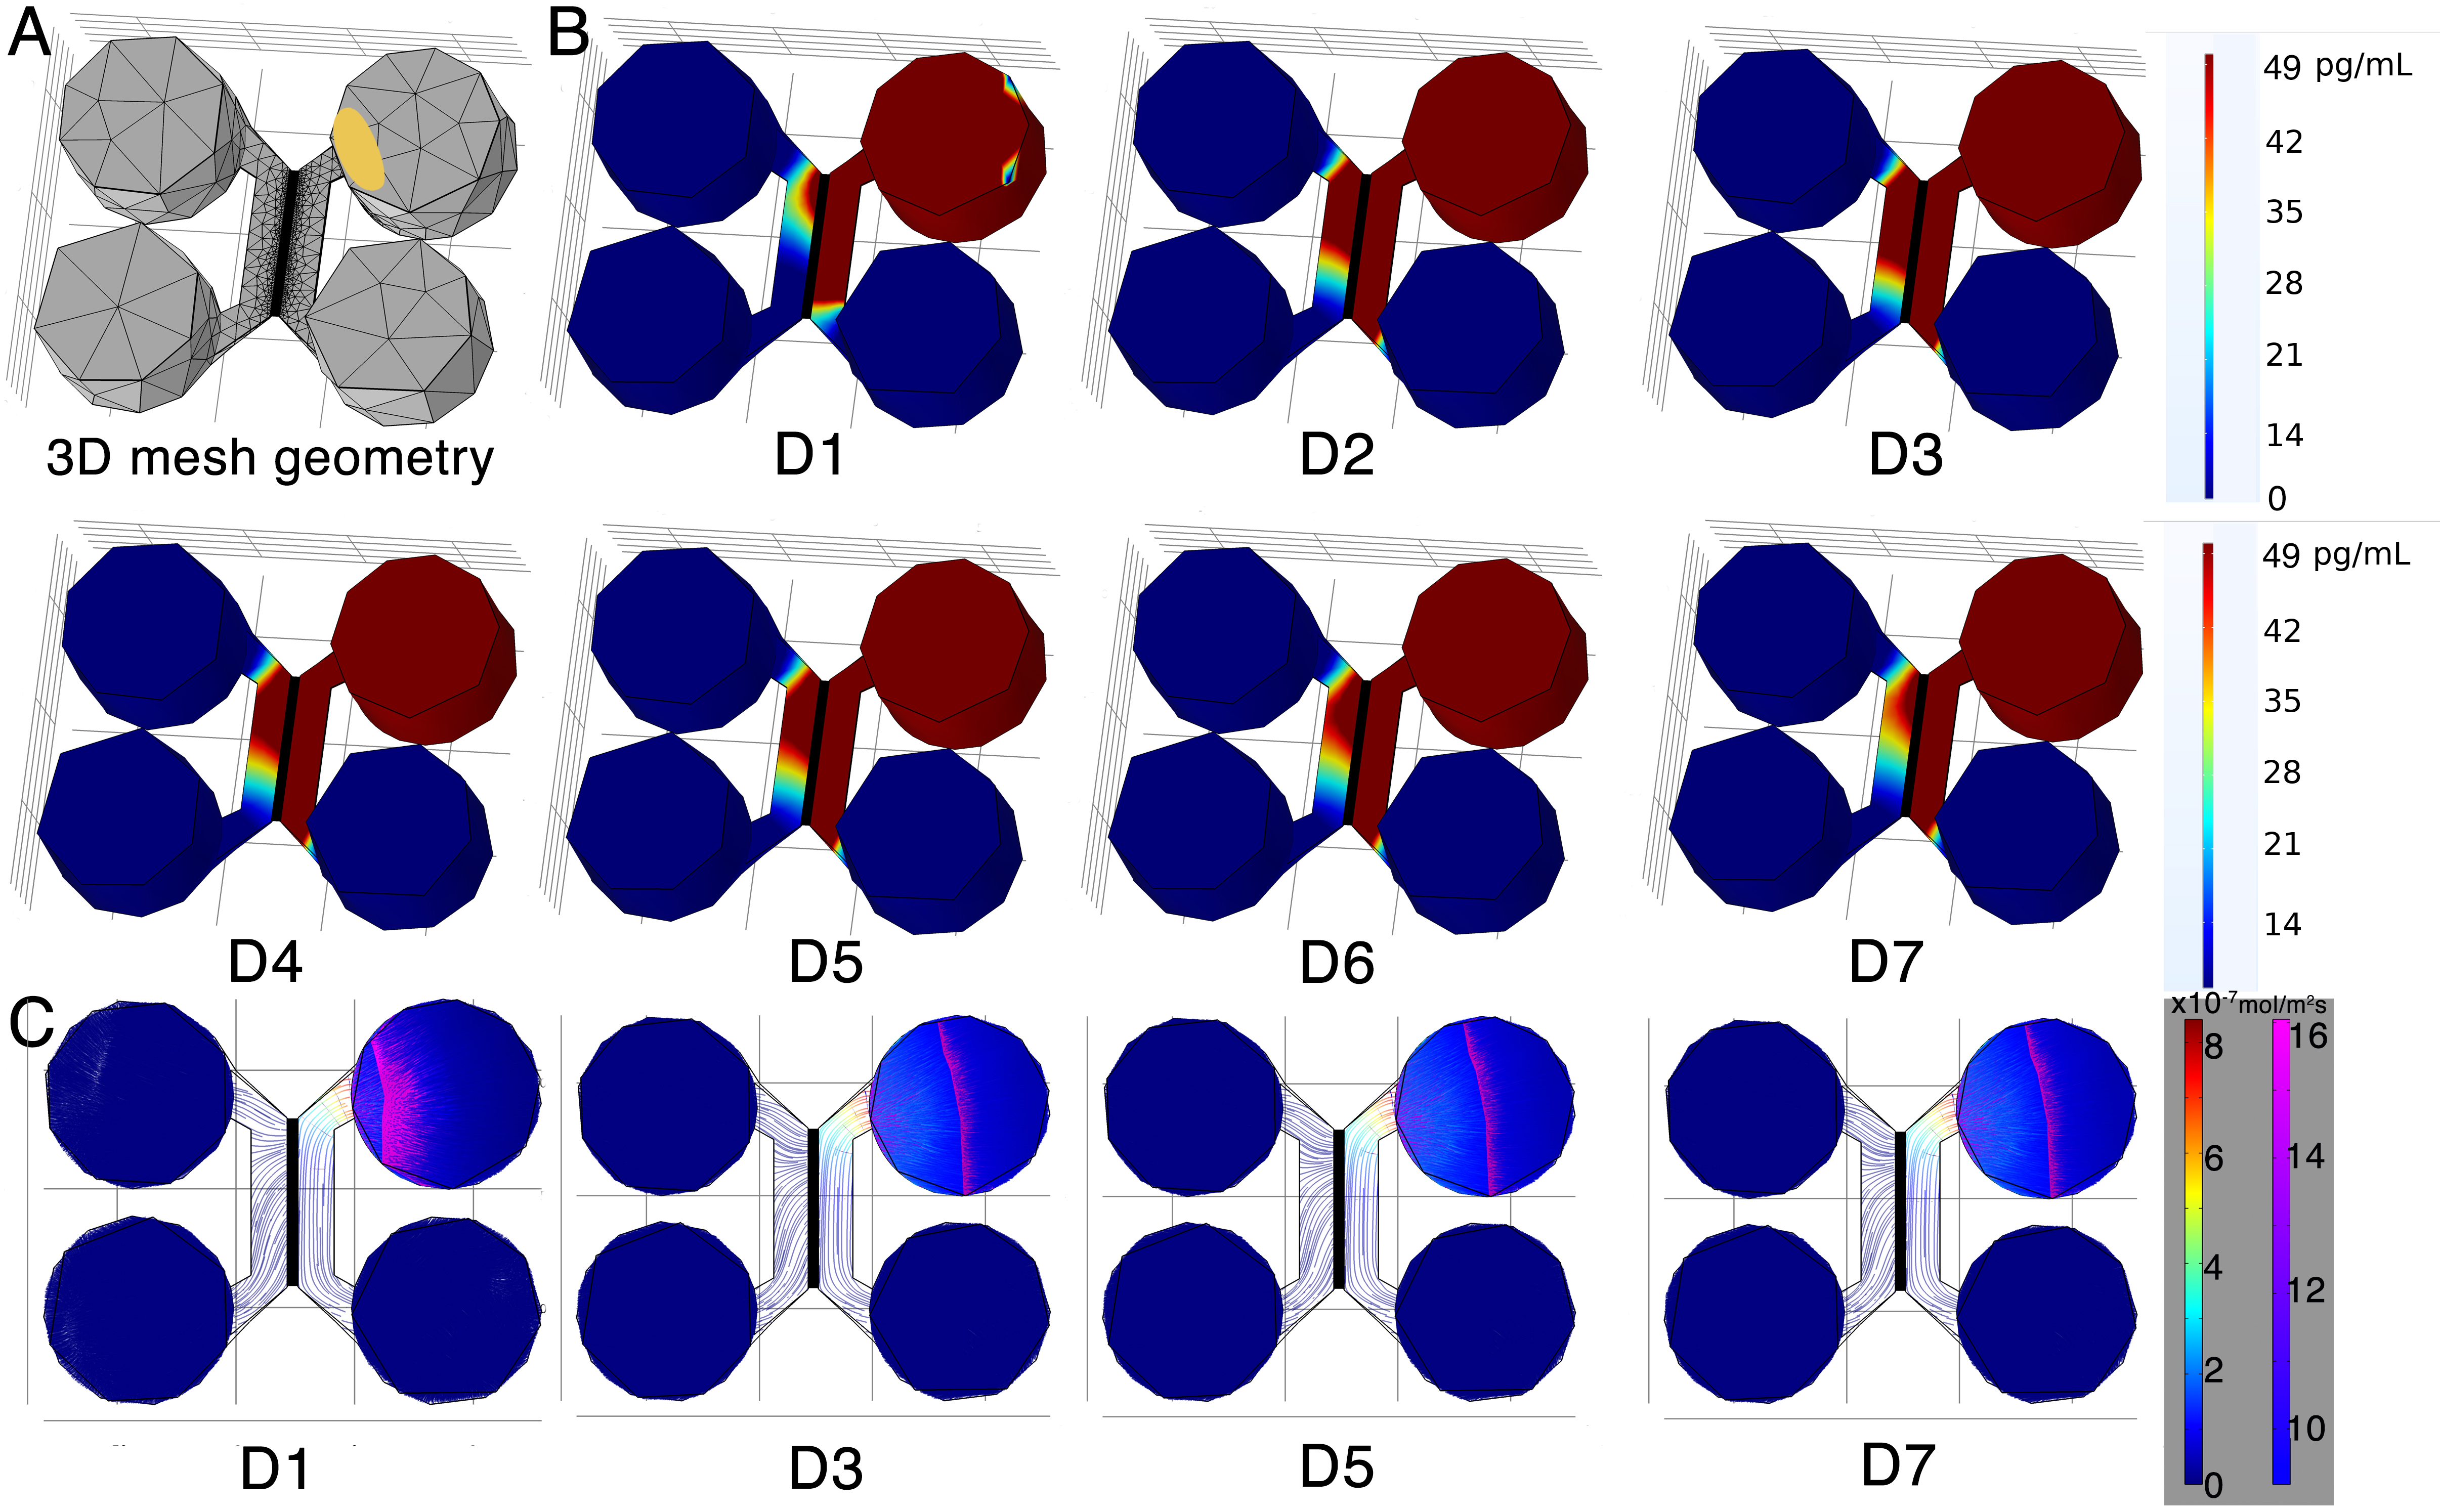
\includegraphics[width=13cm]{Fig_5.jpg}
\end{center}
\caption{(A): 3D mesh geometry of a Xona\textsuperscript{\texttrademark} XC450 created with Autodesk Inventor. A PODS\textsuperscript{\textregistered}-rhBDNF ellipsoid disc is shown in yellow. (B): rhBDNF concentration gradient for 20,000 PODS\textsuperscript{\textregistered}-rhBDNF from D1\textendash D7. Note that the model does not account for media changes during the culture period. The corresponding color map shown has a range from 0 ng/mL to 49 pg/mL. (C): Diffusion flux ($mol/m^{2}s$) was computed using COMSOL Chemical Engineering module on D1, D3, D5, and D7.}
\end{figure}

%%%%%%%%%%%%%%%%%%%%%%%%%%%%%
%Figure 6 result explanation%
%%%%%%%%%%%%%%%%%%%%%%%%%%%%%
The finite element model was then computed for different PODS\textsuperscript{\textregistered}-rhBDNF concentrations and time intervals to empirically optimize the rhBDNF concentration gradient for hPSC-derived ONP differentiation into SGNs as well as directed neurite extension. Figure 6 shows FEM-computed rhBDNF concentration gradients for 20,000 PODS\textsuperscript{\textregistered}-rhBDNF from Day 1\textendash 7. Note that the rhBDNF concentrations were greater throughout D2\textendash 5 to promote the neuronal differentiation and neurite outgrowth observed on D7 (Figure 6B). Computed diffusion flux was uniform throughout D1\textendash 7 (Figure 6C). Also note that highest concentration of rhBDNF released from PODS\textsuperscript{\textregistered}-crystals was greater than 50 pg/mL, the concentration sufficient for otic neuronal differentiation and neurite outgrowth of hPSC-derived ONP 3D spheroids determined in our previously published data \cite{Chang2020}. Optimization of the adequate number of PODS\textsuperscript{\textregistered}-rhBDNF was performed empirically; we also performed FEA with 10,000 and 40,000 PODS\textsuperscript{\textregistered}-rhBDNF. Please see detailed discussion for the empirical optimization in Supplementary Figure S8. 


%%%%%%%%%%%%%%%%%%%%%%%%%
% Figure 7 (HEAT MAP)
%%%%%%%%%%%%%%%%%%%%%%%%%
\begin{figure}
	\begin{center}
		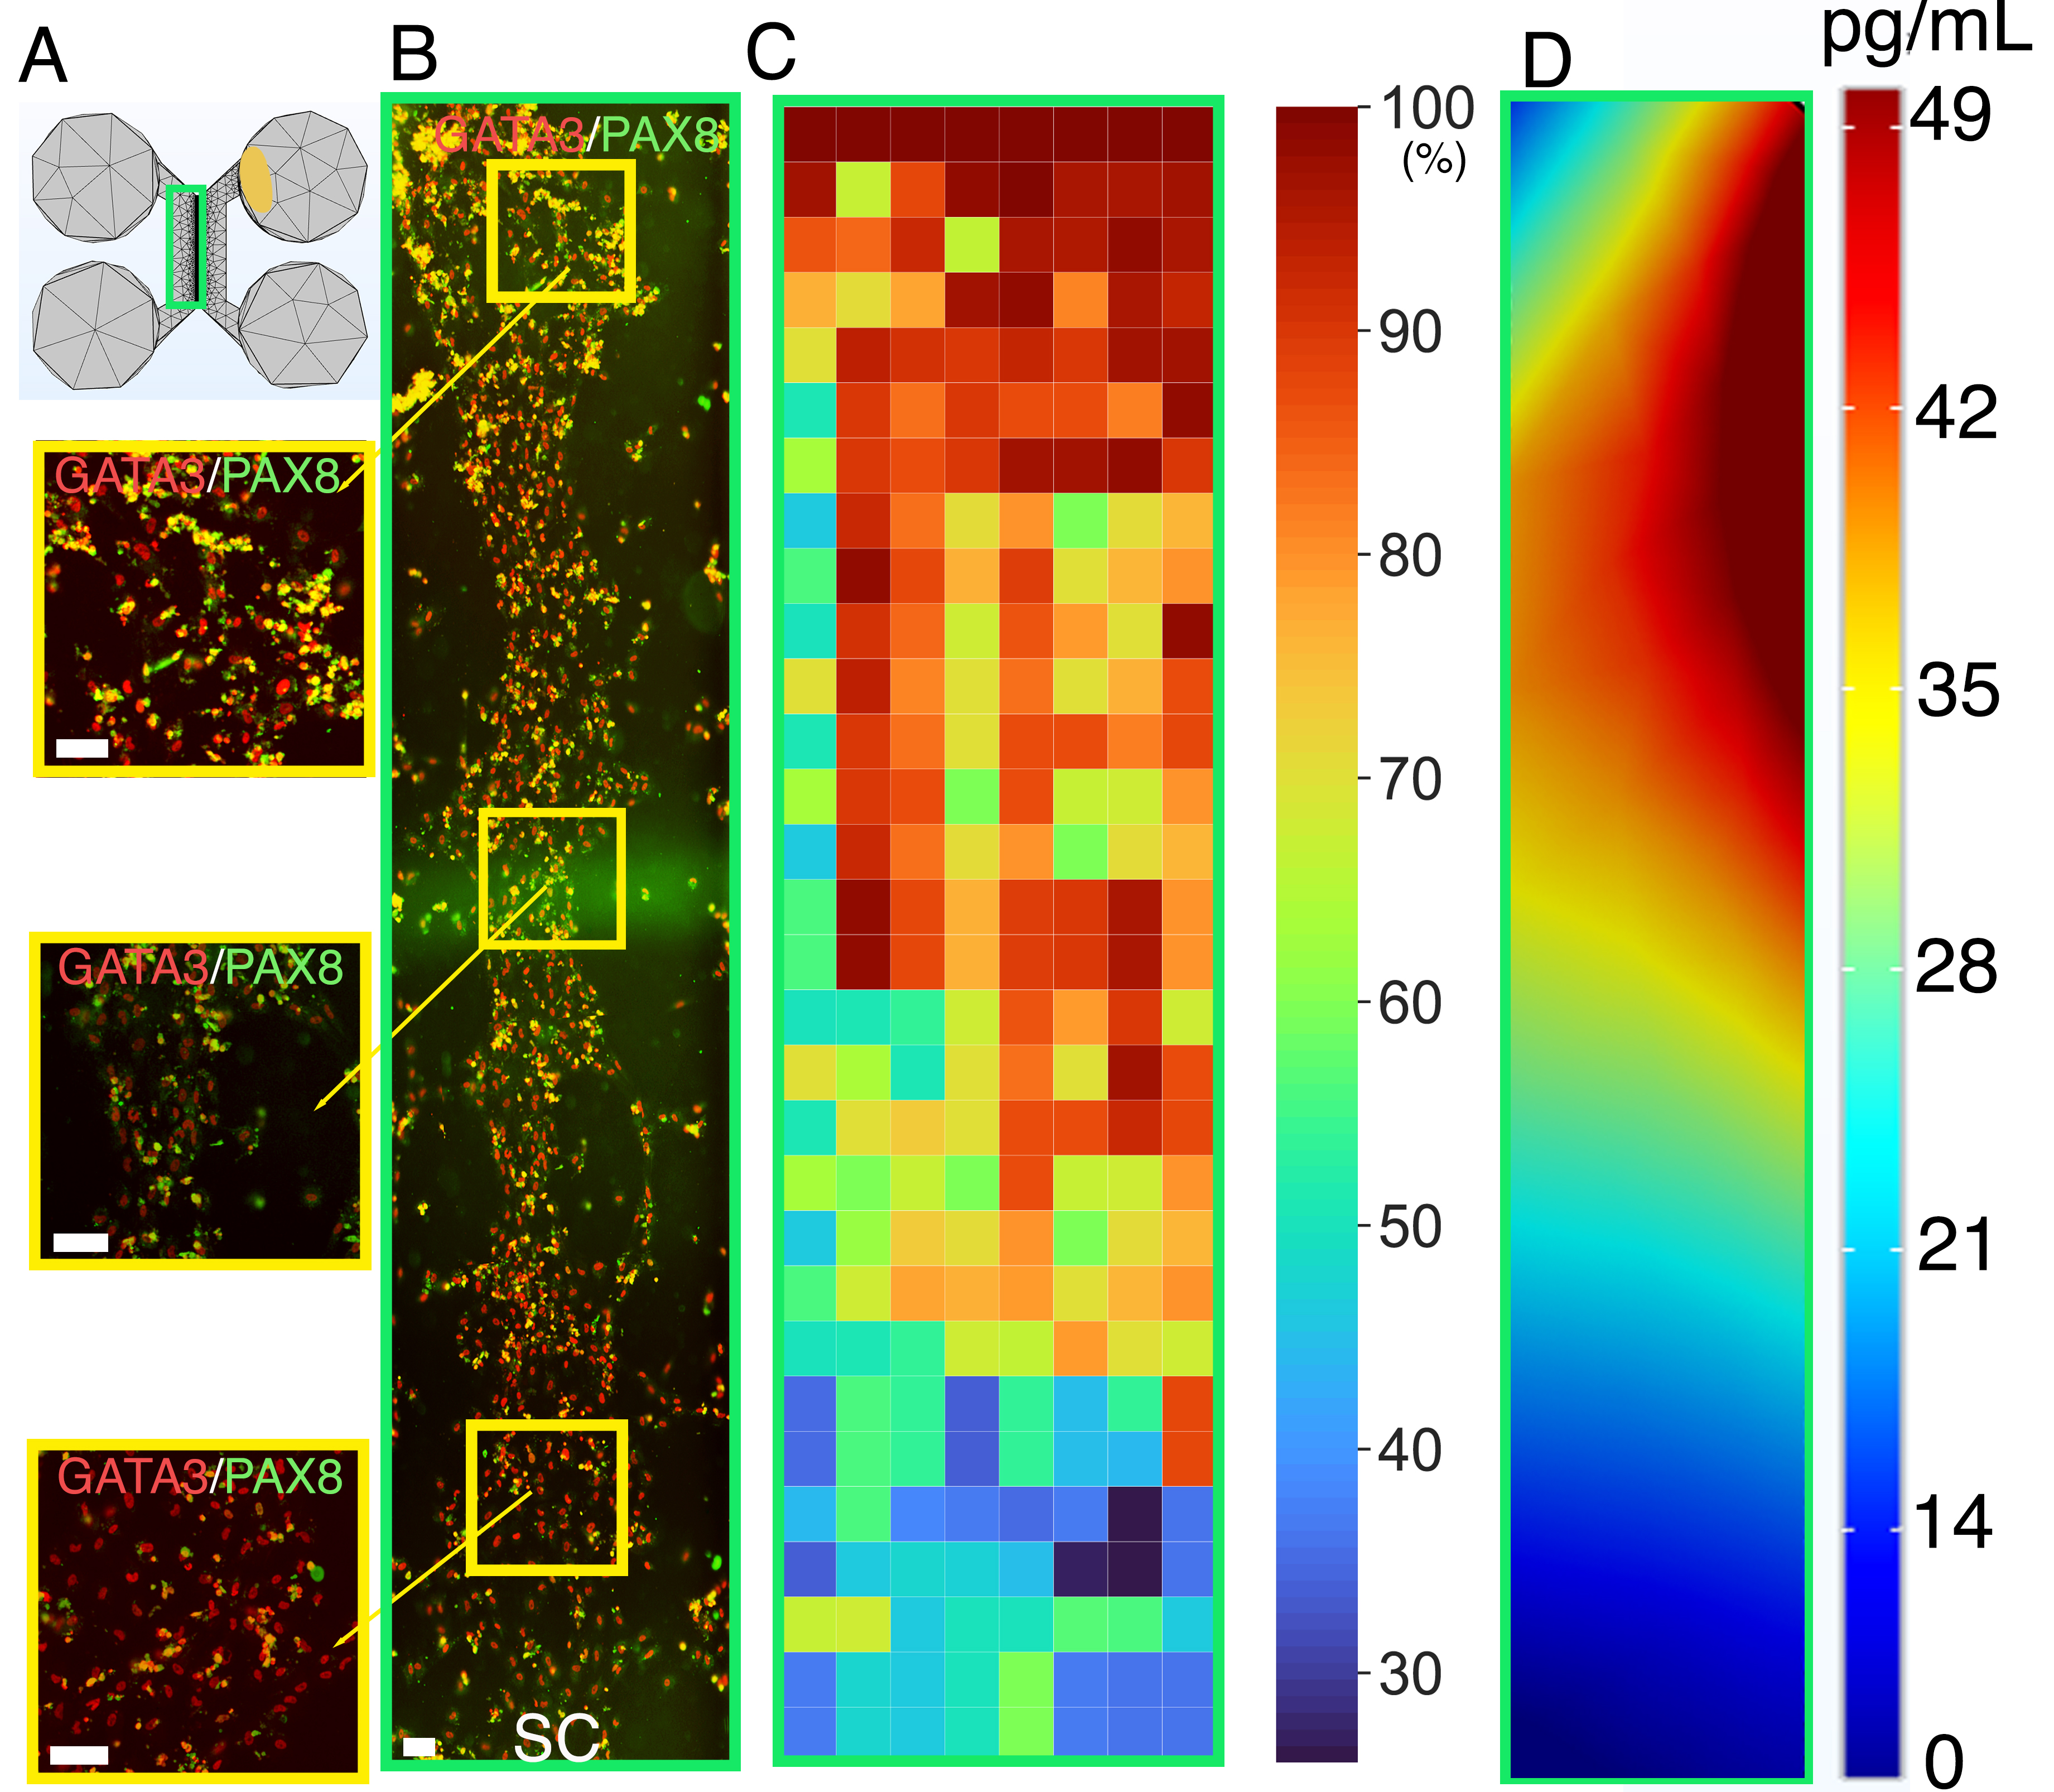
\includegraphics[width=13cm]{Fig_7.jpg}
	\end{center}
	\caption{Human PSC-derived late-stage ONPs grown in a microfluidic device at Day 7 were stained for GATA3 (red) and PAX8 (green). (A): Geometry mesh of the microfluidic device Xona\textsuperscript{\texttrademark} XC450 generated by Autodesk Inventor. The green square indicates the cell seeding location in the somal compartment of the device. An ellipsoid PODS\textsuperscript{\textregistered}-rhBDNF disc is shown in yellow. (B): Cells were analyzed by staining with neuronal markers GATA3 (red) and PAX8 (green). Yellow highlighted regions are magnified on the left. SC: somal compartment. (C): Heat-map representation of double-positivity of hPSC-derived ONPs in the device for GATA3 and PAX8 (n = 3). Double-positivity increases from the lower to the upper portion of the somal compartment, suggesting that the higher BDNF concentration in the upper portion of the device improves differentiation. Scale bar: 100 $\mu$m. (D): Prediction of BDNF concentration gradient released from PODS\textsuperscript{\textregistered}-rhBDNF at seven days in culture using the finite element model.  The corresponding color map is shown with a range from 0\textendash49 pg/mL.
	}
\end{figure}

%%%%%%%%%%%%%%%%%%%%%%%%%%%%%%%%%%%%%%%%
% Figure 7 RESULT
%%%%%%%%%%%%%%%%%%%%%%%%%%%%%%%%%%%%%%%%
To objectively compare the degree of otic neuronal differentiation in the hPSC-derived ONPs, we performed quantitative analysis of PAX8 and GATA3 double-positive cells using immunocytochemistry. We chose PAX8 and GATA3 for this analysis because our previous studies indicated high expression of these protein markers in late-stage ONPs and early-stage SGNs \cite{Heuer2021,Chang2020, Matsuoka2017}. Cells were stained in the somal compartment of the Xona\textsuperscript{\texttrademark} device, highlighted in green in Figure 7A. Figure 7B shows the resulting image of cells in the somal compartment, and a heat-map representation of the percentage of double-positive cells is shown in Figure 7C.
It should be noted here that the heat-map is sensitive to the differences in cell density across channel. This was accounted by averaging the double-positivity across three biological replicates. The heat-map indicates higher double-positivity in the upper region of the somal compartment, which is closest to the PODS\textsuperscript{\textregistered}-rhBDNF disc placement (shown as an orange ellipse in Figure 7A) in the neurotrophin compartment. Double-positivity decreases in the somal compartment as distance from the PODS\textsuperscript{\textregistered}-rhBDNF disc increases, supporting the presence of a rhBDNF neurotrophin gradient as predicted by our computational model (Figure 7D).


%%%%%%%%%%%%%%%%%%%%%%%%%%%%%%%%%%%%%%%%%
% Figure 8 (fig_7.5) hypothetical angles%
%%%%%%%%%%%%%%%%%%%%%%%%%%%%%%%%%%%%%%%%%
\begin{figure}
	\begin{center}
		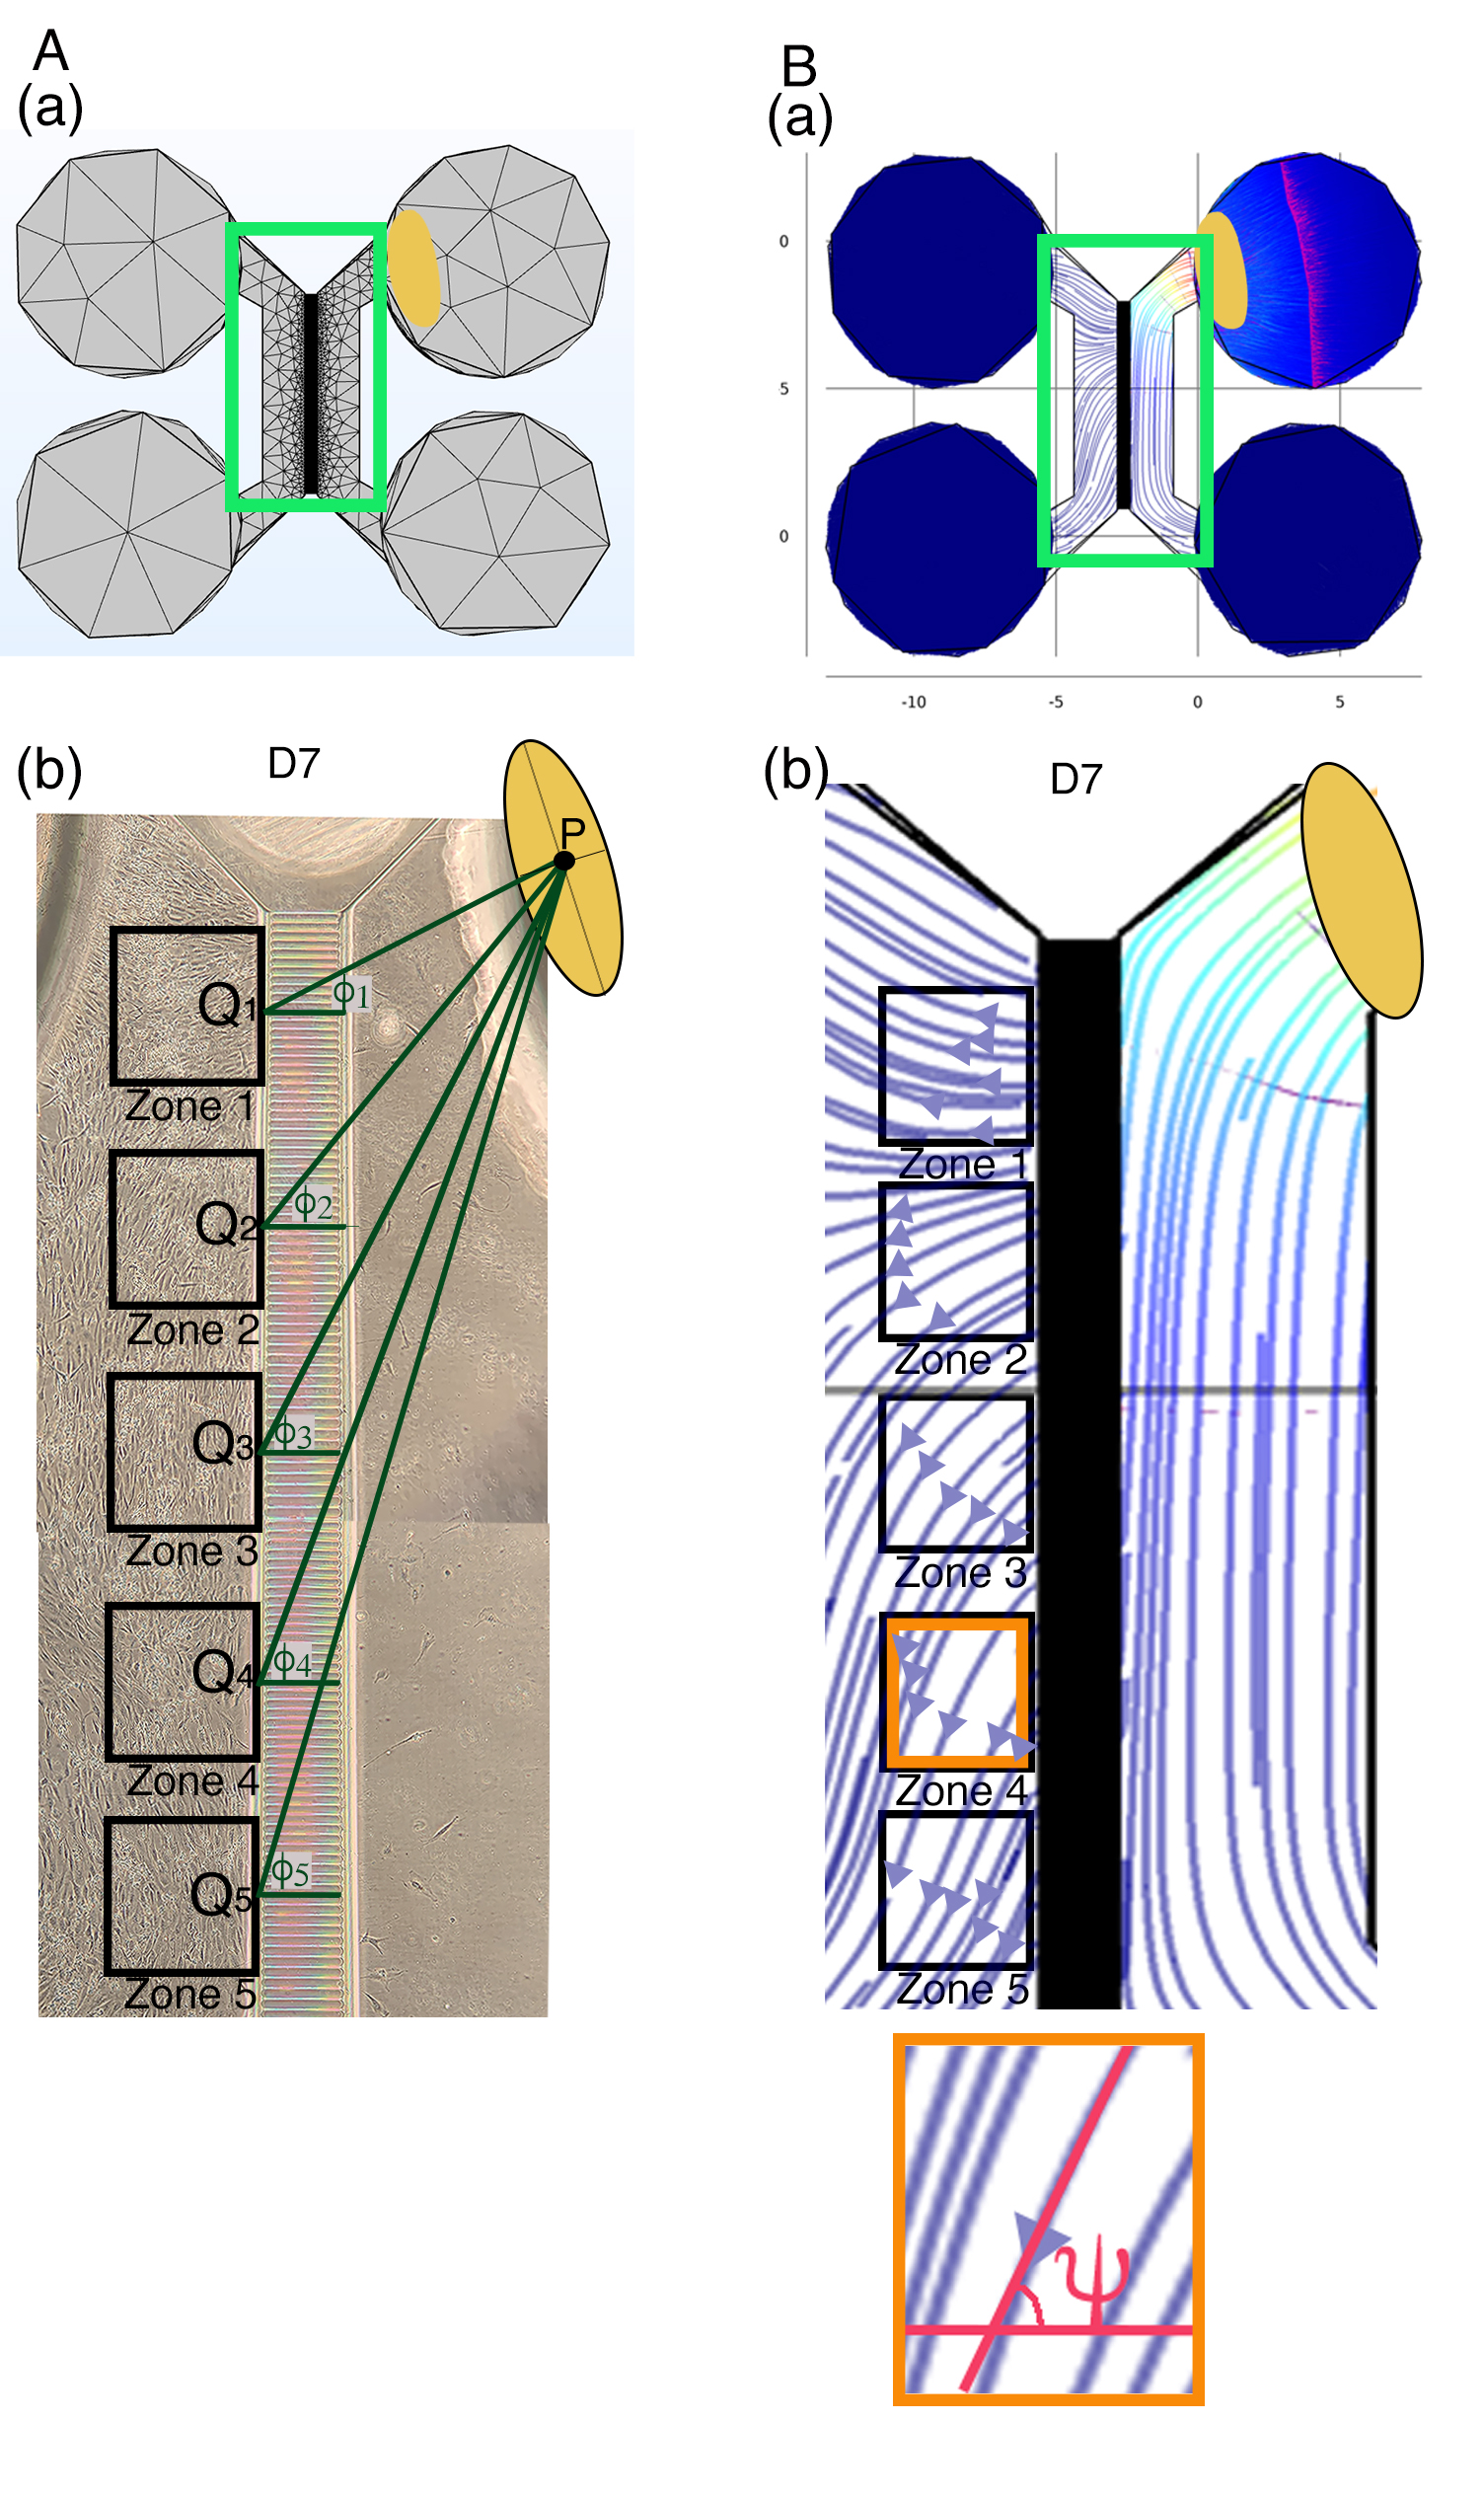
\includegraphics[width=9cm]{Fig_75.jpg}
		% for some LATEX reason, eps was not taken. Used jpeg. 
	\end{center}
	\caption{(A): Defining the Euclidean distance angle (EDA). (a) X-Y plane geometry mesh of a Xona\textsuperscript{\texttrademark} XC450 device. Green square shows the area corresponding to the phase-contrast image below. An ellipsoid PODS\textsuperscript{\textregistered}-rhBDNF disc is shown in yellow. (b) Yellow ellipse once again indicates the location of a disc containing PODS\textsuperscript{\textregistered}-rhBDNF crystals (P: the center of this ellipse). In the somal compartment of the Xona\textsuperscript{\texttrademark} XC450 device, we defined Zone 1\textendash 5, shown in black squares. A line was drawn from the center of the PODS\textsuperscript{\textregistered}-rhBDNF disc (P) to ($Q_{1-5}$) (i.e., the near side to microgroove channels) of a pre-designated square (shown as a black square, zone 1\textendash 5) [i.e.,zone 1\textendash 5]). The Euclidean distance angle (EDA) for zone 1\textendash5 was defined as $\phi_{i}$, $i = 1\textendash 5$. (B): Defining diffusion flux angle (DFA). (a) Diffusion flux in the Xona\textsuperscript{\texttrademark} XC450. Green squared area shows somal and neurotrophin compartments, which are magnified in (b). (b) Magnified image of diffusion flux of Zone 1\textendash 5 in the Xona\textsuperscript{\texttrademark} XC450. Orange highlighted zone (zone 4) was magnified at the bottom of (b), defining the DFA ($\psi$).}
\end{figure}

%%%%%%%%%%%%%%%%%%%%%%%%%%%%%
%Figure 8 result explanation%
%%%%%%%%%%%%%%%%%%%%%%%%%%%%%
\indent We defined two hypothetical directional angles to predict the orientation of hPSC-derived ONPs and neurite growth (Figure 8). The $n$-dimensional Euclidean space, denoted by $\mathbb{R}^{n}$, is a linear vector space in that we can use polar coordinates to compute the directionality of cells and neurites \cite{Axler2015}. Here, we used $n$ = 1 and 2. For one-dimensional Euclidean space ($n$ = 1), we simply drew a line for the Euclidean distance\textemdash the shortest distance between two points as shown in Figure 8A(b) (dark green lines).  The two points were 1) the center point of the PODS\textsuperscript{\textregistered}-rhBDNF disc ($P$) and 2) the mid point of the medial side ($Q_{1-5}$) (i.e., the near side to microgroove channels) of a pre-designated square (shown as a black square, zones 1\textendash 5 in Figure 8), respectively. The Euclidean distance angle (EDA), $\phi_{i}$, was defined as the angle between the horizontal line zero direction and the line $PQ_{i}$ that consists of the Euclidean distance where $i$ = 1 \textendash 5.\\
\indent For two-dimensional Euclidean space ($n$ = 2), we utilized Fick's first law, which dictates that the diffusion flux ($D$) is proportional to the concentration gradient ($C$) \cite{crank1979}. Based on this theorem, the direction of a flow vector can be used to represent the concentration gradient for directionality. We hypothesized here that cell orientation is directionally controlled by the flux vector which is driven by the concentration gradient. Figure 8B shows the flow vectors in the somal compartment at Day 7 computed by the COMSOL Chemical Reaction Engineering module.  We averaged the 10 flow vectors in each of five zones in Figure 8 to compute the diffusion flux angle (DFA), $\psi_{i}$, where $i$ = 1\textendash 5 in Figure 8. To lighten the computational intensity, we reduced the dimension from 3D to 2D to compute diffusion flux. Please see justification in Supplementary Data. All of the computed EDAs and DFAs can be found in Supplementary Table 2. 

%%%%%%%%%%%%%%%%%%%%%%%%%%%%%%%%%%%%%%%%%%%%%%%%%%%%
% Figure 9 (Old version: Fig.8, it is now Figure 9)%
%%%%%%%%%%%%%%%%%%%%%%%%%%%%%%%%%%%%%%%%%%%%%%%%%%%%
\begin{figure}
	\begin{center}
		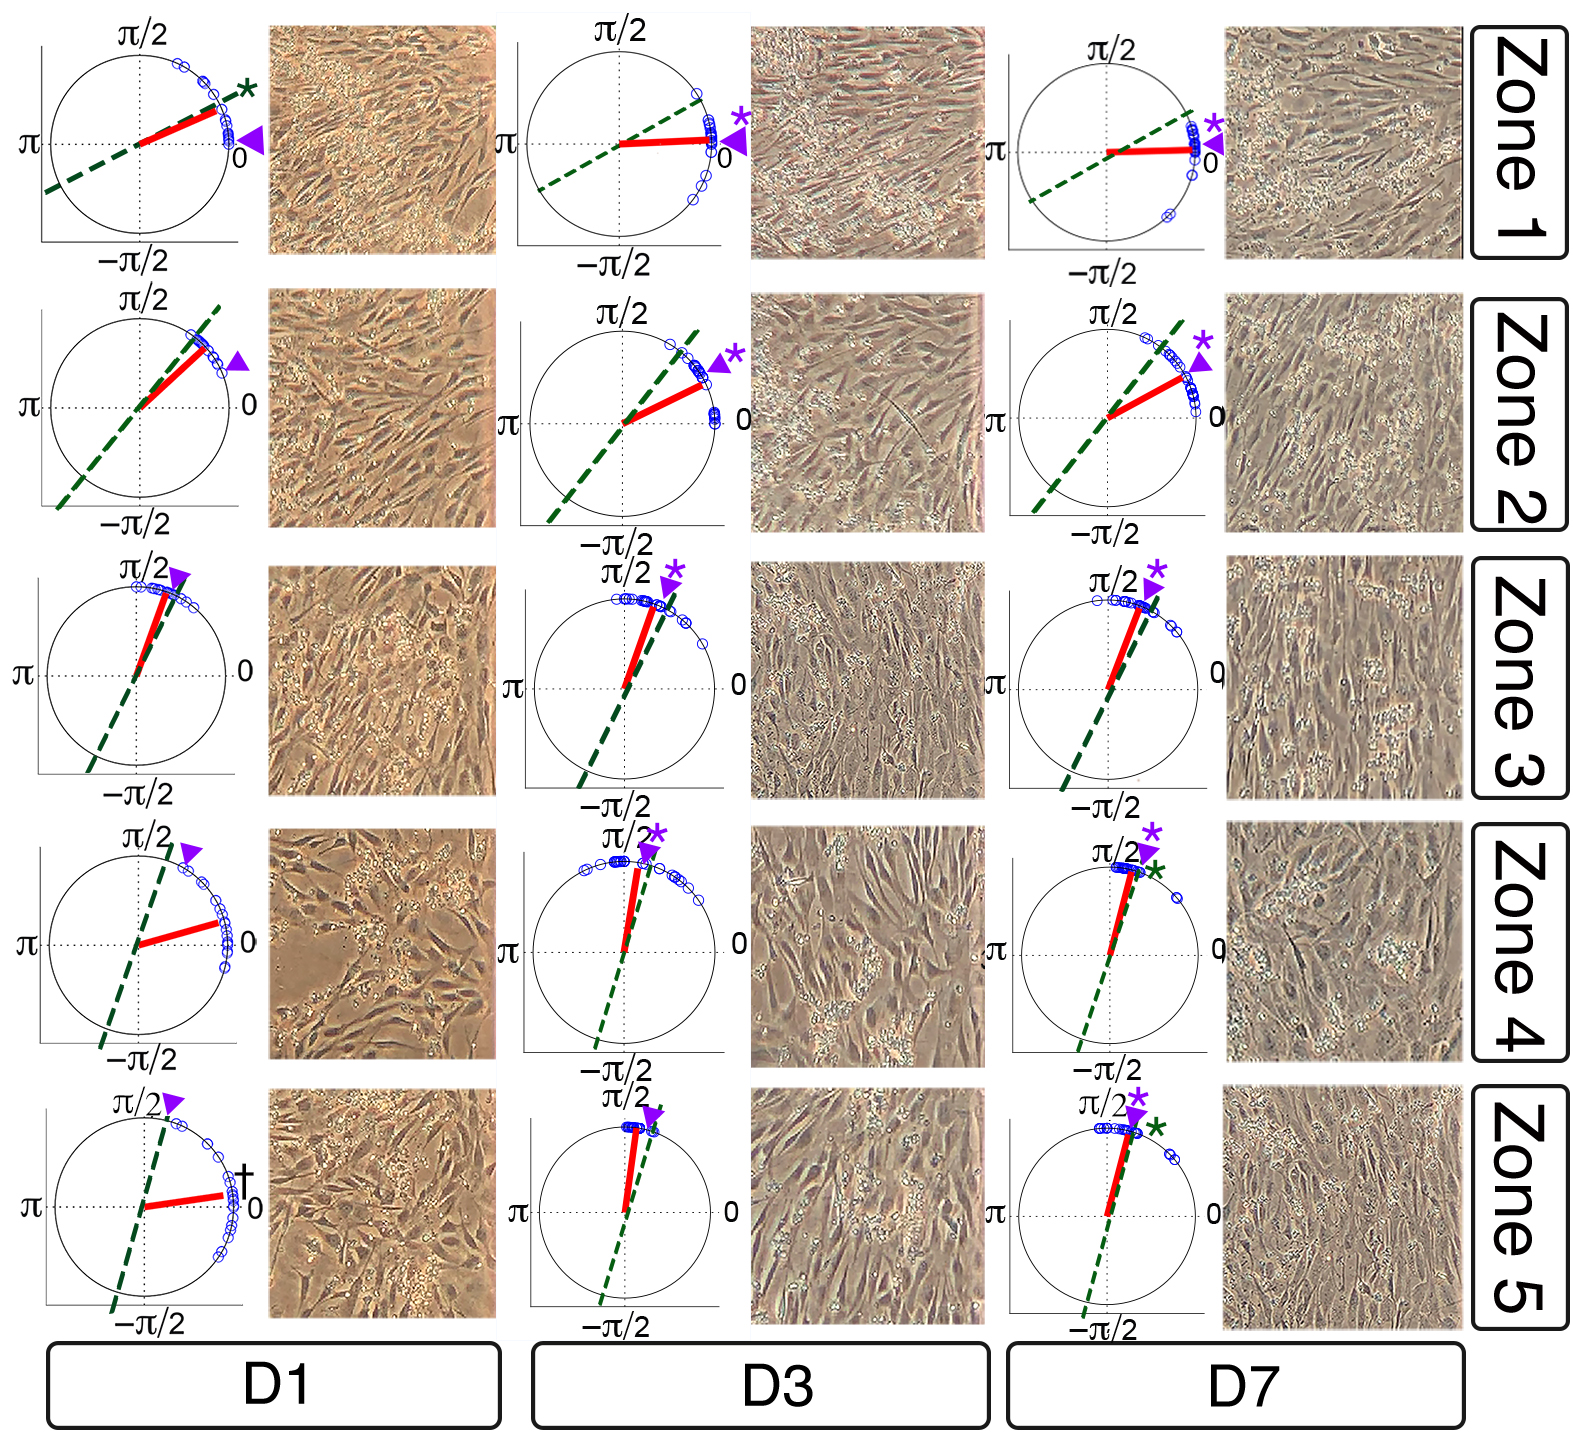
\includegraphics[width=13cm]{Fig_8.jpg}
		% for some LATEXish reason, eps was not taken. Used jpeg. 
	\end{center}
	\caption{Preferred cell orientation analysis. Sequential phase-contrast images of the somal compartment of the Xona\textsuperscript{\texttrademark} XC450 device in zones 1\textendash 5 (see Figure 8) on day 1 (D1), day 3 (D3), and day 7 (D7). A corresponding polar histogram indicates preferred orientation of hPSC-derived ONPs in an angle (0\textendash2$\pi$ radians) in blue circles. Mean vector angle is shown in red line. Green dotted line shows Euclidean Distance Angle (EDA) and purple triangle indicates Diffusion Flow Angle (DFA). $\dagger$ symbol indicates that $p$ value $>$ 0.01. $\ast$ symbol indicates that the mean vector angle fits within the 95\% confidence internal ($\alpha$ $<$ 0.05.)}
\end{figure}

%%%%%%%%%%%%%%%%%%%%%%%%%%%%%
%Figure 9 result explanation%
%%%%%%%%%%%%%%%%%%%%%%%%%%%%%
\indent Figure 9 shows time-series of microscopic phase-contrast photomicrographs obtained on Day 1, 3, and 7 in the five zones in the Xona\textsuperscript{\texttrademark} XC450. Each preferred orientation of any given cell was computed and then plotted on a polar diagram (blue circle). Mean vector angle (MVA, shown in red line on Figure 9) and median vector angle were computed. All of the polar diagrams in Figure 9 show that preferred orientation of hPSC-derived ONPs distribute in an unimodal distribution. We also confirmed that a von Mises distribution is appropriate for these sets of data (See Supplementary Figure S9). We, therefore, then tested further to see if the cells had tendency to be oriented to a certain direction. To test this hypothesis, we used the Rayleigh test of uniformity to evaluate whether there is statistical evidence of circular directionality \cite{Batschelet1981}. Computed $p$ values for all the 15 conditions were less than 0.05, demonstrating that all of the conditions had statistically significant directionality. To further validate whether the observed angles have a tendency to cluster around the two hypothetical angles (i.e., EDA and DFA), we then performed the V test. Once again, $p$ values for all 15 conditions were less than 0.05 except one (Zone 5 on Day 1), re-demonstrating that most of the conditions had statistically significant tendencies to cluster around the EDAs and DFAs. Additionally, we performed one sample test for the mean vector angle, which is similar to a one sample t-test on a linear scale. There was only one condition (Zone 1, day 1) that was statistically significant for EDA, whereas most of the conditions on Day 3 and 7 were statistically significant for DFA. Therefore, our results here demostrated that hPSC-derived ONPs had greater tendency to cluster around DFA than EDA. All computed statistical values are shown in Supplementary Table S2.

%%%%%%%%%%%%%%%%%%%%%%%%%%%%
% Figure 10 (IHC migration)%
%%%%%%%%%%%%%%%%%%%%%%%%%%%%
\begin{figure}
	\begin{center}
		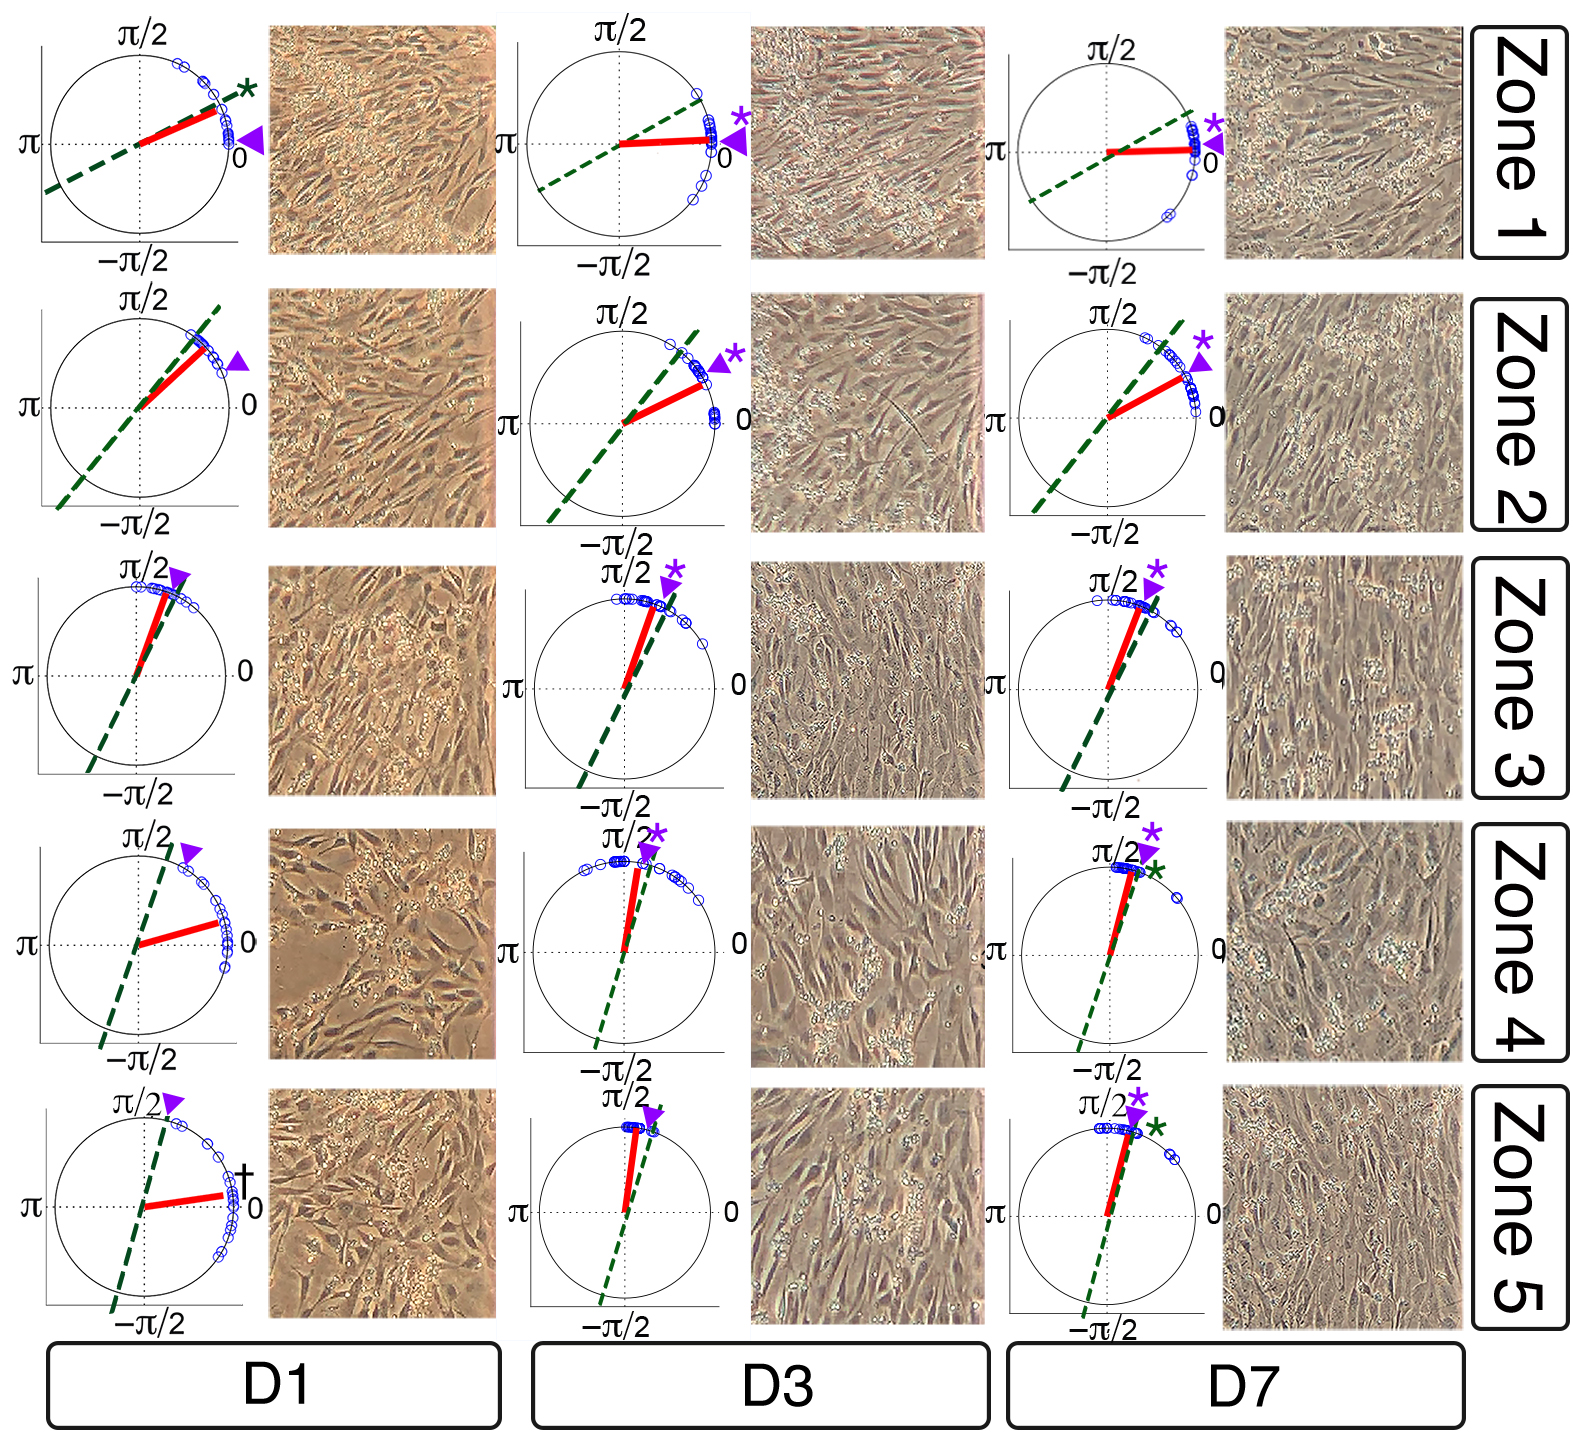
\includegraphics[width=11cm]{Fig_9.jpg}
	\end{center}
	\caption{(A): Immunohistochemistry of hPSC-derived ONPs cultured in the Xona\textsuperscript{\texttrademark} XC450 for seven days with $\beta$-III-Tubulin (pink fluorescence) and DAPI (blue fluorescence). A green line was drawn from the center of the BDNF disc (P) to the mid point of each of three pre-determined squares (Regions 1\textendash 3) in the somal compartment to define Euclidean Distance Angle (EDA: $\phi^{`}_{i}$, $i$ =1 \textendash 3). Green square: somal compartment (SC); yellow square:  microgroove channels (MGC); white square: Neurotrophin compartment (NTC). High-power magnified images of the NTC and SC are shown. An ellipsoid PODS\textsuperscript{\textregistered}-rhBDNF disc is shown in yellow. P: the center of the disc.(B): Polar histogram of  neurite directional angles of hPSC-derived ONPs in the Xona\textsuperscript{\texttrademark} XC450 at Day 7 (D7). The two longest neurites were measured. EDA: green dotted line. DFA: purple triangle. (C): (a) Right: Polar histogram of neurite directional angles of hPSC-derived ONPs cultured with 20 ng/mL of recombinant human BDNF for seven days. Left: Corresponding photomicrograph of immunocytochemistry with $\beta$-III tubulin (pink) and DAPI (blue). ()b) Right: Polar histogram of neurite directional angles of hPSC-derived ONPs cultured with 800,000 of PODS\textsuperscript{\textregistered}-rhBDNF for seven days. Left: Corresponding photomicrograph of immunocytochemistry with $\beta$-III tubulin (pink) and DAPI (blue). (D):  A circular plot of neurite directional angle of hPSC-derived ONPs in Region 1\textendash 3. Once again, the two longest neurites were plotted on a unit circle. Right column: Original directional angle distribution. Left column: the method of doubling the angle applied to the original data. Each datum point is shown as a blue circle. Mean vector angle is shown as a red line. Green dotted line shows Euclidean Distance Angle (EDA) and purple triangle indicates Diffusion Flow Angle (DFA). $\ast$ symbol indicates that the mean vector angle fits within the 95\% confidence internal ($\alpha$ $<$ 0.05.)}
\end{figure}

%%%%%%%%%%%%%%%%%%%%%%%%%%%%%%$
% Figure 10 Result explanation%
%%%%%%%%%%%%%%%%%%%%%%%%%%%%%%$
To evaluate the direction of neurites of hPSC-derived ONPs, we first defined EDA in Region 1-3 ($\phi^{\prime}_{j}$, $j$ =1 \textendash 3) (Figure 10A) and DFA ($\psi^{\prime}_{j}$, $j$ =1\textendash 3); similarly defined $\phi_{i}$ and $\psi_{i}$ as in Figure 8. All of the EDAs and DFAs defined here can be found in Supplementary Table S3. Polar histograms of the neurite direction angle in Regions 1\textendash 3 indicated that the two longest neurites were bimodal in nature (Figure 10B).  In contrast, polar histograms of those cultured with rhBDNF (negative control) and 800,000 PODS\textsuperscript{\textregistered}-BNDF (positive control) did not indicate bimodal distribution\textemdash the neurites did not show directionality (Figure 10C). The Rayleigh test of uniformity for both the positive and negative control were greater than 0.05, demonstrating that both of the conditions had no statistically significant directionality (Supplementary Table S3: highlighted in green). We also analyzed the direction of the neurites using circular statistics. To obtain more realistic mean vector angles, we doubled each angle and reduced the multiples modulo 360\degree. In circular statistics, the bimodal distributed data can be transformed into a unimodal data by doubling the angle \cite{Batschelet1981}. The mean vector angles in Figure 10D (right column) indicates the situation where the vectors were canceled out between the two groups of angles distributed in a bimodal fashion, resulting in inaccurate representation. A circular plot in Figure 10D (right column) showed doubled angles, representing actual representation of the neurite vector angles. In all of the three regions, the Reyleigh test and V test for EDA and DFA indicated directionality (Supplementary Table S3). One sample test for the mean vector angles in Region 1\textendash 3 indicated that they were not statistically different from DFA, but all of the three mean vector angles were statistically different from EDA. 

%%%%%%%%%%%%%%%%%%%%%%%%%%%%%%%%%%%%%%%%%%%%%%%%%%%%
% Figure 11 (IHC neurite growth assay and migration)
%%%%%%%%%%%%%%%%%%%%%%%%%%%%%%%%%%%%%%%%%%%%%%%%%%%%
\begin{figure}
	\begin{center}
		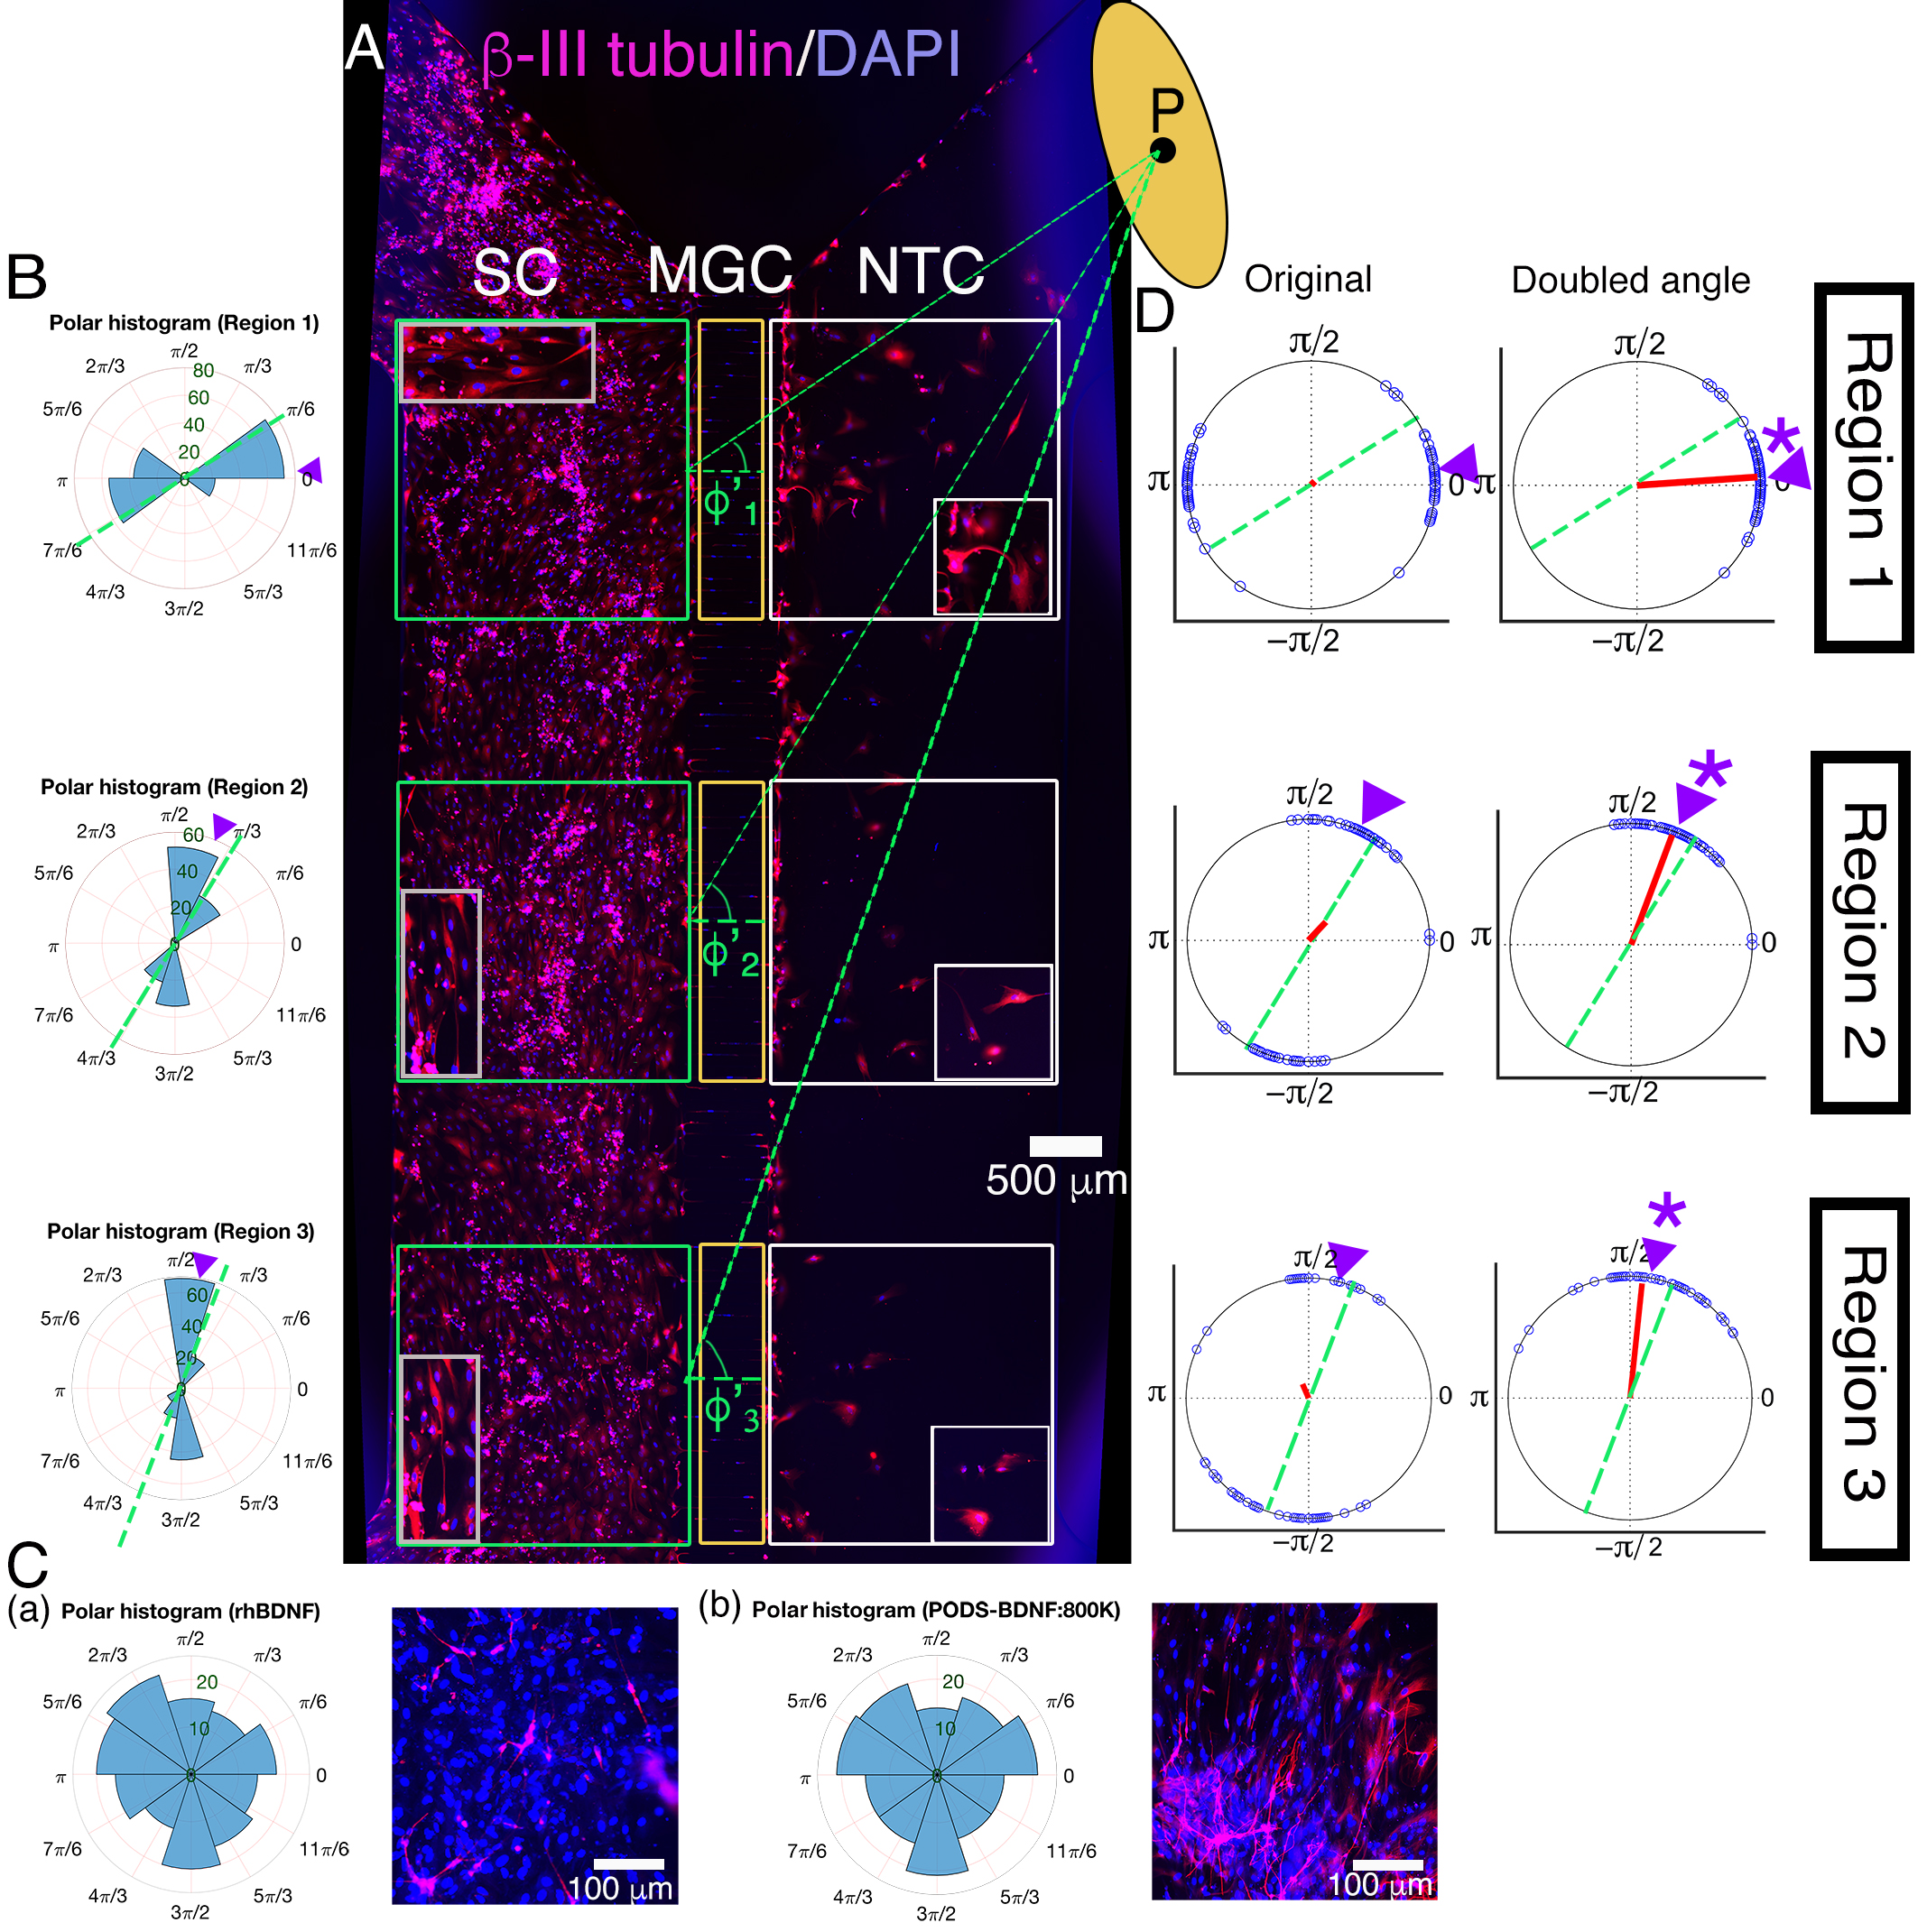
\includegraphics[width=12cm]{Fig_10.jpg}
	\end{center}
	\caption{Human PSC-derived late-stage ONPs in the microfluidic device were stained with $\beta$-III tubulin (red) and DAPI (blue) to measure cell migration. (A): Late-stage ONPs stained after seven days in culture (a) with regions highlighted and magnified in the somal compartment (b), microgroove channels (c), and neurotrophin compartment (d). SC: somal compartment, MGC: microgroove channels, NTC: neurotrophic compartment. An ellipse-shaped PODS\textsuperscript{\textregistered}-rhBDNF disc is shown in yellow. Scale bar (a): 500 $\mu$m;(b)\textendash(d): 100 $\mu$m. (B): Quantitative analyses of cell migration and neurite extension in devices using recombinant human BDNF, 800,000 PODS\textsuperscript{\textregistered}-rhBDNF, or 20,000 PODS\textsuperscript{\textregistered}-rhBDNF. * : $p$ $<$ 0.05, **: $p$ $<$ 0.01, ***: $p$ $<$ 0.001.}
\end{figure}


%%%%%%%%%%%%%%%%%%%%%%%%%%%%%%
%Figure 11 Result explanation%
%%%%%%%%%%%%%%%%%%%%%%%%%%%%%%
We also stained the devices for $\beta$-III tubulin to track neurite growth and extension across the micro-groove channels as well as cell migration in three selected regions (Figure 10A). The location of the PODS\textsuperscript{\textregistered}-rhBDNF disc in relation to the regions of interest in Figure 11A is indicated by a yellow circle. Quantitative analyses were performed and summarized in Figure 11B. Our data indicate that neurite length is dependent on rhBDNF concentration, with greater amounts of PODS\textsuperscript{\textregistered}-rhBDNF promoting longer neurite growth (Figure 11B(a)). Lesser amounts of PODS\textsuperscript{\textregistered}-rhBDNF, however, are necessary to create an appropriate concentration gradient. In the presence of 20,000 PODS\textsuperscript{\textregistered}-rhBDNF, both neurite extension into the microchannels and cell migration into the neurotrophin compartment are greatest in the region closest to the BDNF source and decrease further from the PODS\textsuperscript{\textregistered}-rhBDNF (Figure 11B(b,c)). Cell migration is dependent on the distance from the source of BDNF, thus suggesting the presence of a BDNF gradient as predicted by our model. Note that the Xona microchannels intended to prevent from migration across channels. 


%%%%%%%%%%%%%%%%%%%%%%%
\section {Discussion}%%
%%%%%%%%%%%%%%%%%%%%%%%
\subsection{Challenges of neurotrophin treatment in the inner ear}  
This is a proof-of-concept study for the realization of a neurotrophic strip to ascertain its scientific/technological parameters in a controlled \textit{in vitro} environment. Neurotrophin gradients have been studied in multiple contexts \cite{Keefe2017,Awad2015,Hollis2011}. However, it has not been feasible to reliably provide, and maintain, such a gradient to neurons \textit{in vivo}, primarily because of challenges including failure to provide a sustainable source. Furthermore, while neurotrophin treatment has been recognized as a potential treatment for sensorineural hearing loss, there has not been long-term clinical success in this avenue to date. Most recent relevant clinical trials used adeno-associated virus (AAV2) to deliver BDNF to the brain \cite{Nagahara2018}. Although compelling, this treatment does not attempt to precisely control the concentration of BDNF, which could potentially interfere with normal functions in the target organ \cite{Croll1999}. Furthermore, this treatment may not be applicable to the inner ear, as the procedure is MR-guided\textendash infeasible in the inner ear. In this study, we used PODS\textsuperscript{\textregistered}-rhBDNF to provide and maintain a neurotrophic gradient in a controlled manner. Our result indicated 20,000 PODS-rhBDNF allowed for a rhBDNF neurotrophin gradient such that hESC-derived ONPs survived, differentiated toward human SGNs, and also established directional neurite outgrowth in a microfludic device. Furthermore, our proposed solution has the potential to be translated to clinical practice; in addition to its proven natural self-sustainability, we have shown that transplantation of PODS-rhBDNF is met with little immune rejection when embedded in a nanofibrillar cellulose hydrogel in mice \cite{Chang2020}.

\subsection{Microfluidic device-generated gradient}
We used a microfluidic device to advance our understanding of directional neurite growth and otic neuronal differentiation in response to a rhBDNF concentration gradient \cite{dravid2020}. Among many \textit{in vitro} concentration gradient sustaining culture devices, microfluidic devices have overcome many of the deficits that conventional platforms (i.e., the Boyden chamber, Dunn chambers, or compartmentalized diffusion chambers) face \cite{dravid2020}. Conventional platforms tend to be sub-optimal in manipulating small volumes of fluid at the order of microliters. Growth factors and proteins are used in minute amounts in our microfluidic device, and cultured stem cells are able to interact with endogenous factors at biologically relevant concentrations. As mentioned earlier, this micro-environment more accurately represents \textit{in vivo} conditions. The Xona\textsuperscript{\texttrademark} device can be used to create and sustain a three-dimensional concentration gradient over time (duration dependent on the half-life of the molecule) because of its microchannel array.  The device limits convective flow in the gradient-forming areas by introducing microgroove channels that generate high fluidic resistance, thereby limiting flow to diffusion. The high resistance of the microchannel array also prolongs diffusion across them, thereby increasing gradient formation and elongation of the gradient. These features motivated us to generate a FEM, which predicted the rhBDNF gradients associated with different numbers of PODS\textsuperscript{\textregistered}-BDNF crystals. Note, however, that this environment is geometrically different from the micro-environment in the inner ear\textendash a mesh geometry of the cochlea will be needed to compute the PODS\textsuperscript{\textregistered}-BDNF crystal number for the next step of this study. 

\subsection {BDNF and Polyhedrin protein} 
Over the course of past 20\textendash 30 years, it has been established that BDNF mediates survival and differentiation activities on SGNs by binding and activating the thyrosine kinase receptor kinase B (TrkB), a member of the larger family of Trk receptors \cite{green2012}. Numerous studies have reported that BDNF can palliate SGN degeneration in ototoxically deafened animals, a widely accepted model for retrograde trans-synaptic SGN degeneration secondary to hair cell destruction \cite{Gillespie2003,Pettingill2008,Yamagata2004,Zanin2014}. Additionally, it has been confirmed that there is a positive correlation between SGN counts and CI performance \cite{Seyyedi2014}. It is then safe to presume that treating CI recipients with BDNF would enhance overall CI performance, by preserving SGNs and their neurites. However, simply introducing rhBDNF into the inner ear poses significant hurdles.  Although promising, human BDNF treatment has not been currently implemented in the inner ear. Unsuccessful BDNF treatment can be explained by several factors \cite{Henriques2010}. 

\indent The blood half-life of BDNF protein is extremely short, only 1–10 min in the plasma \cite{Poduslo1996,Sakane1997} and one hour in CSF \cite{Soderquist2009}. The BDNF's high degradation rate would require continuous replenishment, impractical for clinical use. Furthermore, introduction of a homogeneous solution of BDNF would promote nondirectional neurite growth where directed neurite growth is essential for designing our new-generation bioactive CI, as depicted in Figure 1A. Directing neurite growth towards the CI electrode array is pivotal in the ultimate goal of enhancing performance through the narrowing of the electrode-neuron gap. The PODS\textsuperscript{\textregistered} system precludes the phenomena by its localized, gradual release of growth factor. The steady supply of BDNF from a localized origin not only creates a concentration gradient, but maintains it over time. As seen in Figures 4\textendash 6, we were able to perform a finite element analysis based on data we collected describing the chemical release kinGtics and molar ratio of PODS\textsuperscript{\textregistered}-BDNF system. It is clearly visible that the slow-release nature of PODS\textsuperscript{\textregistered}-BDNF results in a concentration gradient over the course of Day 1\textendash 7 (Figure 5). 

\indent It should be noted that our FEM assumes free diffusion of the rhBDNF protein. In biological cell-culture conditions, BDNF released from PODS\textsuperscript{\textregistered}-BDNF has tendency to adhere to the walls of the culture device because BDNF is a ``sticky" protein of about 27 kDa (mature BDNF dimer) and it is positively charged under physiological conditions (isoelectric point, pI = 9.4) \cite{Sasi2017}. As such, the physio-chemical properties of BDNF have made the recombinant protein difficult to diffuse. This phenomenon was observable in preliminary data where the ONPs failed to survive past 1\textendash 3 days of culture (data not shown). To circumvent this issue we infused the culture media with a carrier protein (i.e., BSA), hypothesizing that the albumin would act as a carrier for the released BDNF and allow for free diffusion throughout the microfluidic device \cite{Li2010}. This hypothesis is supported by our sets of biological verification data (Figures 7\textendash 11) that clearly shows that hPSC-derived ONPs responded to the modification by exhibiting the expected cell body orientation, unidirectional neurite extension, and neurite length. Note that albumin is the single protein found in highest concentrations in the perilymph \cite{Swan2009}, therefore, a carrier protein will not be needed in our future \textit{in vivo} study.  

\subsection{Intracellular signaling initiated by Thyrosine kinase B receptor}
Another issue we need to consider in interpretation of our results is the intracellular cell signaling mechanism elicited by rhBDNF. Human BDNF (mature dimeric form) binds with high affinity to its TrkB receptor. The binding of BDNF to a TrkB receptor has proven to have significant importance for the proneuronal effects of BDNF \cite{green2012}. Upon binding BDNF, TrkB dimerizes, and activates intrinsic kinase activities and other complex set of intracellular signaling cascades, which is beyond the scope of this study. However, it should be noted that activation of TrkB receptor by neurotrophin binding causes the TrkB protein to be internalized in endosomes on the cellular membrane \cite{Numakawa2010}. Endosomes can then be transported to the soma. Therefore, the proneuronal effects of rhBDNF in our results might have highly depended on the status of TrkB receptors on the cell membrane of hPSC-derived ONPs. Our previous study has demonstrated that strong expression of a TrkB receptor on derived ONPs \cite{Matsuoka2017}, however, more detailed studies on TrkB receptors on hPSC-derived ONP and SGNs will be needed.

\subsection{Degradation of PODS\textsuperscript{\textregistered} crystals by protease}
In cell culture, degradation of PODS\textsuperscript{\textregistered}-rhBDNF is likely due to the activity of cell-secreted proteases. The proteases break down the peptide bonds of the encasing polyhedrin protein, creating openings in the structure to allow release of the rhBDNF. Therefore, the presence of proteases is imperative for the proper utilization of the PODS\textsuperscript{\textregistered} crystals. Additionally, these proteases are responsible for the degradation of the released BDNF. Because stem cells are not present in the culture media used for the PODS\textsuperscript{\textregistered} degradation kinetics experiments, we infused the media with 10\% FBS, which naturally contains proteases, to promote polyhedrin degradation, BDNF release, and BDNF degradation to attain results that more accurately describe \textit{in vitro} events. Moreover, since the cells and PODS are initially segregated into separate compartments within the culture device, cell-secreted proteases are unlikely to reach and degrade the PODS in time to support ONP survival and differentiation. Infusion of FBS was therefore required in these experiments as well. In clinical use, however, we presume that cell-secreted proteases will be readily present in the inner ear and would therefore preclude the need for artificial supplementation.

\subsection{A concept design: Neurotrophic strip}
The plateau in CI performance in treatment of sensorineural hearing loss has driven researchers to develop innovative supplementary treatment strategies to push the field past this hurdle. Our approach strives to directly address the issue at its core: the electrode-neuron gap, which can lead to serious implications include low spatial frequency resolution and high power consumption. We can use our data as a launchpad for the neurotrophic strip (NS). The NS is a biointerface concept that integrates an extended-release source of growth factor to facilitate a protein gradient. Implanted in conjunction with the CI, it acts as a bridge between the extant SGNs and implanted late-ONPs grown on the electrode itself. The NS would promote survival of both cell populations, differentiation of the late ONP implants, promote directional neurite growth and synaptogenesis between the two, effectively creating a neuronal network between the patient and the implanted CI. Each electrode would be able to stimulate cell bodies at exceptionally high resolution, essential for greater intonation differentiability (required for effective social interaction and music appreciation) and so, increased quality of life for millions. Our successful outcomes are essential to make a neurotrrophic strip feasible in \textit{in vivo} environment. 

\subsection{The limitations of this study and future direction}
There are some limitations associated with this study.  First, the reduction of spacial dimension to 2D  for diffusion modeling certainly affected the flux vector, which determines the predicted concentration vector. Given that the thickness (i.e., Z-axis) of the microfluidic device was 100 $\mu$m, we estimated that the effect was minimal. In the future, we plan to use PSC-derived 3D spheroids in a somal compartment so that flux vector and concentration gradient vector can more accurately model the cell behavior. In this way, we will be able to circumvent the need to reduce diffusion calculations to 2D for computation performance in the modeling. 

\indent Secondly, we required to generate a model in that the BDNF's biological transportation phenomenon from a PODS\textsuperscript{\textregistered}-rhBDNF disc to a somal compartment of a Xona\textsuperscript{\texttrademark} device. Note that in this model, we focused on the major dependent variable, BDNF concentration gradient to model the biological phenomenon. Other physical variables to promote cell migration, otic neuronal differentiation, and neurite growth were not take into consideration. These variables include electotaxis (electrical potential), durotaxis (matrix's stiffness [i.e., laminin 511 in our case]) \cite{Gentile2016}, mechanotaxis (cell strain), and lastly cell migration by random walk \cite{berg1983}. In our future study, we will take these variables into consideration to more accurately represent the migration and neurite growth of hPSC-derived ONPs. 

\indent Insufficient contrast between cells and background in phase contrast images led to inaccuracies in cell orientation computation for some images. To address this issue, poor quality images were disregarded in the quantitative analysis. We occasionally used manual measurement for accuracy. Our future study may entail automated time-series cell analysis, which would allow more accurate measurement. Also, another way to address this issue would be with a cell membrane staining in the future. 

\indent While 20,000 of PODS\textsuperscript{\textregistered}-rhBDNF were necessary for hPSC-derived ONPs for otic neuronal differentiation and directional neurite outgrowth, this condition may not be sufficient. For instance, it is still not known whether the effects of other neurotrophic factors such as Neurotrophin-3 and Glial cell line-derived neurotrophic factor could have a positive effect on ONP growth \cite{green2012, li2017, Schulze2020}. We are planning to investigate these neurotrophic factors in the future. Other factors that could have an impact on directional neurite growth include endogenous factors secreted from hPSC-derived ONPs. While our previous study demonstrated that hPSC-derived ONPs only secreted negligible amount of BDNF that were detected by ELISA \cite{Chang2020}, currently we do not have any data on other neurotorphic factors or other molecules that could have affected directional neurite growth in the inner ear. We chose BDNF first to study because the most intensively studied neurotrophic factor in the field of hearing research is BDNF \cite{green2012}. Previous studies have indicated that neurotrophic supports of SGNs are mainly from BDNF and neurotrophin-3 (NT-3) \cite{green2012,Sasi2017}. Therefore, the potential confounding effect of the secretions of other neurotrophic factors and molecules secreted from derived SGNs are likely NT-3, for which further investigation is necessary in the future.  

\indent Despite the aforementioned limitations associated in this study, the present results generated BDNF concentration gradient, condition of which is necessary for hPSC-derived ONPs to differentiate into the otic lineage (i.e., SGNs) and also promoted directional neurite extension towards the POD-BDNF disc. The technique will allow us to control neurite direction of transplanted hPSC-derived ONPs in the inner ear. We will harness this method in our design of a bioactive CI. 

%\subsection{otic neuronal differentiaion vs. neurite growth concentration} 
% KEVIN, 18) "threshold gradient value of 20 ng/mL/mm was required, while 50 ng/mL/mm induced branching" -can be included in our disussion (Dravid 2020)
% 10/2/21 - will write a sentence regarding this - will be added to the end of statistical/biological discussion subsection

\section* {Conclusions}
We were able to generate BDNF concentration gradient, enabling survival, neuronal differentiation toward SGNs, and directed neurite extension of hPSC-derived ONPs. The technique will allow us to control neurite direction of transplanted hPSC-derived ONPs in the inner ear. This proof-of-concept study provides a step toward next-generation bioacitve CI technology. 

\section* {Acknowledgment}	
This work was supported by the American Otological Society Clinician Scientist Award (AJM), the Triological Society/American College of Surgeons Clinician Scientist Award (AJM), the Department of Otolaryngology of Northwestern University (AJM), the NIH (NIDCD) K08 Clinician Scientist Award K08DC13829-02 (AJM), and the Office of the Assistant Secretary of Defense of Health Affairs through the Hearing Restoration Research Program (Award \#: RH170013:WU81XWUH-18-0712). Imaging work was performed at the Northwestern University Center for Advanced Microscopy, which is generously supported by NCI CCSG P30 CA060553 awarded to the Robert H. Lurie Comprehensive Cancer Center, for which we thank Peter Dluhy, Constadina Arvanitis, Ph.D., David Kirchenbuechler, Ph.D., and Wensheng (Wilson) Liu, M.D.  Some of microfluidic device experiments were performed in the Analytical bioNanoTechnology (ANTEC) Core Facility of the Simpson Querrey Institute at Northwestern University, which is supported by the Soft and Hybrid Nanotechnology Experimental (SHyNE) Resource (NSFECCS-1542205). We thank Shreyas Bharadwaj (Cornell University), Kyle Coots (Midwestern University), Andrew Oleksijew (the University of Nebraska), Duncan Chadly (California Institute of Technology), and Shun Kobayashi (the University of Texas at Austin) for their contribution to the earlier phases of this project. We thank Sara Dunlop (Department of Neurology, Northwestern University), and Dr. Jacqueline Bond (the University of California San Diego) for assistance in Western Blot and SDS-Page gels. We also thank Dr. Georgia Minakaki (Department of Neurology, Northwestern University) on assistance in ELISA. Finally, our thanks and appreciation go to our collaborator, Dr. Christian Pernstich (Cell Guidance Systems), for continuous support and stimulating discussions on this project since 2015. 

% using a watershed plugin
%need citation here. 
% Soille, P., and Vincent, L.M. Determining watersheds in digital pictures via flooding simulations. In: Kunt M, editor. Visual Communications Image Process.’90 Fifth a Ser. [Internet]. Lausanne, Switzerland, 1990.
% so as to extract the individual cell contours.



\bibliography{mybibfile}
\end{document}
